% IEEE Transactions on Quantum Engineering (TQE) manuscript.
% Build: `make paper` from the repository root (latexmk or tectonic).
% Every result number is a macro from numbers.tex, generated from results/ by
% `python -m experiments.paper_numbers`; `make check-paper` fails if it is stale.
\documentclass[journal]{IEEEtran}

\usepackage{amsmath,amssymb,amsthm}
\usepackage{graphicx}
\usepackage{booktabs}
\usepackage{multirow}
\usepackage[table]{xcolor}
\usepackage{cite}
\usepackage[hyphens]{url}
\usepackage{algorithm}
\usepackage{algpseudocode}
\usepackage[hidelinks]{hyperref}

\graphicspath{{../figures/}}
% Generated by `python -m experiments.paper_numbers` from results/. Do not edit:
% `make check-paper` fails if this file differs from a fresh regeneration.
\newcommand{\BtcAdv}{13{,}578}
\newcommand{\BtcLot}{0.001}
\newcommand{\BtcBeta}{1.52}
\newcommand{\BtcBetaSe}{0.16}
\newcommand{\BtcBetaRsq}{0.17}
\newcommand{\BtcHalfSpread}{0.0008}
\newcommand{\BtcSigma}{3.75}
\newcommand{\BtcVolPerMin}{9.4}
\newcommand{\BtcImpactBars}{23{,}024}
\newcommand{\LinkAdv}{1{,}156{,}589}
\newcommand{\LinkLot}{0.1}
\newcommand{\LinkBeta}{1.19}
\newcommand{\LinkBetaSe}{0.10}
\newcommand{\LinkBetaRsq}{0.08}
\newcommand{\LinkHalfSpread}{0.56}
\newcommand{\LinkSigma}{5.97}
\newcommand{\LinkVolPerMin}{803.2}
\newcommand{\LinkImpactBars}{23{,}024}
\newcommand{\LinkAdvMillions}{1.157}
\newcommand{\NumDevDays}{16}
\newcommand{\NumTestDays}{12}
\newcommand{\TestFirstDay}{2026-08-07}
\newcommand{\TestLastDay}{2026-08-18}
\newcommand{\DevFirstDay}{2026-07-22}
\newcommand{\DevLastDay}{2026-08-06}
\newcommand{\TestCommit}{f64de87}
\newcommand{\TestCommitClean}{clean}
\newcommand{\TestWallTime}{250}
\newcommand{\EvalSizes}{0.1\% or 0.5\%}
\newcommand{\EvalHorizons}{60 or 240}
\newcommand{\ParticipationCapPct}{25}
\newcommand{\NumStartTimes}{6}
\newcommand{\NumCells}{4}
\newcommand{\HybridClipLow}{0.5}
\newcommand{\HybridClipHigh}{2}
\newcommand{\NumTestWindows}{72}
\newcommand{\NumPrimaryComparisons}{12}
\newcommand{\PrimaryMinHolm}{1.00}
\newcommand{\PrimaryMinRawP}{0.10}
\newcommand{\PrimaryMinMean}{$-$0.27}
\newcommand{\PrimaryMaxMean}{+0.22}
\newcommand{\PrimaryNumSignificant}{0}
\newcommand{\BtcMaxAbsCi}{0.38}
\newcommand{\BtcNumEquivalent}{6}
\newcommand{\LinkMeanCiHalfWidth}{1.45}
\newcommand{\BtcQuboTwapMean}{$-$0.10}
\newcommand{\BtcQuboTwapCi}{[$-$0.38, 0.18]}
\newcommand{\BtcQuboTwapP}{0.53}
\newcommand{\BtcQuboTwapHolm}{1.00}
\newcommand{\BtcQuboVwapMean}{$-$0.03}
\newcommand{\BtcQuboVwapCi}{[$-$0.09, 0.03]}
\newcommand{\BtcQuboVwapP}{0.44}
\newcommand{\BtcQuboVwapHolm}{1.00}
\newcommand{\BtcQuboAcMean}{$-$0.03}
\newcommand{\BtcQuboAcCi}{[$-$0.09, 0.03]}
\newcommand{\BtcQuboAcP}{0.45}
\newcommand{\BtcQuboAcHolm}{1.00}
\newcommand{\BtcHybridTwapMean}{0.00}
\newcommand{\BtcHybridTwapCi}{[$-$0.25, 0.27]}
\newcommand{\BtcHybridTwapP}{0.92}
\newcommand{\BtcHybridTwapHolm}{1.00}
\newcommand{\BtcHybridVwapMean}{+0.08}
\newcommand{\BtcHybridVwapCi}{[0.00, 0.17]}
\newcommand{\BtcHybridVwapP}{0.10}
\newcommand{\BtcHybridVwapHolm}{1.00}
\newcommand{\BtcHybridAcMean}{+0.08}
\newcommand{\BtcHybridAcCi}{[0.00, 0.17]}
\newcommand{\BtcHybridAcP}{0.10}
\newcommand{\BtcHybridAcHolm}{1.00}
\newcommand{\LinkQuboTwapMean}{$-$0.15}
\newcommand{\LinkQuboTwapCi}{[$-$1.64, 1.16]}
\newcommand{\LinkQuboTwapP}{0.51}
\newcommand{\LinkQuboTwapHolm}{1.00}
\newcommand{\LinkQuboVwapMean}{$-$0.07}
\newcommand{\LinkQuboVwapCi}{[$-$1.04, 0.89]}
\newcommand{\LinkQuboVwapP}{0.99}
\newcommand{\LinkQuboVwapHolm}{1.00}
\newcommand{\LinkQuboAcMean}{+0.22}
\newcommand{\LinkQuboAcCi}{[$-$1.76, 2.03]}
\newcommand{\LinkQuboAcP}{0.16}
\newcommand{\LinkQuboAcHolm}{1.00}
\newcommand{\LinkHybridTwapMean}{$-$0.27}
\newcommand{\LinkHybridTwapCi}{[$-$2.02, 1.13]}
\newcommand{\LinkHybridTwapP}{0.37}
\newcommand{\LinkHybridTwapHolm}{1.00}
\newcommand{\LinkHybridVwapMean}{$-$0.19}
\newcommand{\LinkHybridVwapCi}{[$-$1.28, 0.78]}
\newcommand{\LinkHybridVwapP}{0.80}
\newcommand{\LinkHybridVwapHolm}{1.00}
\newcommand{\LinkHybridAcMean}{+0.10}
\newcommand{\LinkHybridAcCi}{[$-$1.78, 1.86]}
\newcommand{\LinkHybridAcP}{0.18}
\newcommand{\LinkHybridAcHolm}{1.00}
\newcommand{\PrimaryTableRows}{\multirow{6}{*}{BTC} & QUBO $-$ TWAP & $-$0.10 & [$-$0.38, 0.18] & [$-$0.29, 0.08] & 0.53 & 1.00 \\
 & QUBO $-$ VWAP & $-$0.03 & [$-$0.09, 0.03] & [$-$0.09, 0.04] & 0.44 & 1.00 \\
 & QUBO $-$ AC & $-$0.03 & [$-$0.09, 0.03] & [$-$0.09, 0.04] & 0.45 & 1.00 \\
 & Hybrid $-$ TWAP & 0.00 & [$-$0.25, 0.27] & [$-$0.21, 0.21] & 0.92 & 1.00 \\
 & Hybrid $-$ VWAP & +0.08 & [0.00, 0.17] & [$-$0.01, 0.17] & 0.10 & 1.00 \\
 & Hybrid $-$ AC & +0.08 & [0.00, 0.17] & [$-$0.01, 0.17] & 0.10 & 1.00 \\
\midrule
\multirow{6}{*}{LINK} & QUBO $-$ TWAP & $-$0.15 & [$-$1.64, 1.16] & [$-$1.69, 1.09] & 0.51 & 1.00 \\
 & QUBO $-$ VWAP & $-$0.07 & [$-$1.04, 0.89] & [$-$0.75, 0.62] & 0.99 & 1.00 \\
 & QUBO $-$ AC & +0.22 & [$-$1.76, 2.03] & [$-$1.71, 2.22] & 0.16 & 1.00 \\
 & Hybrid $-$ TWAP & $-$0.27 & [$-$2.02, 1.13] & [$-$2.03, 1.09] & 0.37 & 1.00 \\
 & Hybrid $-$ VWAP & $-$0.19 & [$-$1.28, 0.78] & [$-$0.92, 0.48] & 0.80 & 1.00 \\
 & Hybrid $-$ AC & +0.10 & [$-$1.78, 1.86] & [$-$1.90, 2.05] & 0.18 & 1.00 \\}
\newcommand{\SensMinMean}{$-$0.55}
\newcommand{\SensMaxMean}{+0.26}
\newcommand{\SensMinJointHolm}{1.00}
\newcommand{\SensNumComparisons}{48}
\newcommand{\SensNumCiExcludeZero}{4}
\newcommand{\SensExclMean}{+0.14}
\newcommand{\SensExclCi}{[0.02, 0.28]}
\newcommand{\RiskLinkQuboTwapMean}{$-$3.8}
\newcommand{\RiskLinkQuboTwapCi}{[$-$8.1, $-$0.4]}
\newcommand{\RiskLinkQuboAcMean}{+2.1}
\newcommand{\RiskLinkQuboAcCi}{[$-$0.7, 5.0]}
\newcommand{\RiskMinHolm}{0.59}
\newcommand{\BtcAcTwapMean}{$-$0.08}
\newcommand{\BtcAcTwapCi}{[$-$0.35, 0.21]}
\newcommand{\LinkAcTwapMean}{$-$0.37}
\newcommand{\LinkAcTwapCi}{[$-$2.65, 1.95]}
\newcommand{\NumTestOrders}{288}
\newcommand{\BtcSpreadImpact}{0.16}
\newcommand{\BtcStdMin}{43}
\newcommand{\BtcStdMax}{43}
\newcommand{\BtcFillMin}{95}
\newcommand{\BtcFillMax}{96}
\newcommand{\BtcMeanShortfallMin}{4.83}
\newcommand{\BtcMeanShortfallMax}{4.93}
\newcommand{\BtcOppMin}{4.66}
\newcommand{\BtcOppMax}{4.77}
\newcommand{\BtcTimingMin}{0.00}
\newcommand{\BtcTimingMax}{0.04}
\newcommand{\BtcModelCostMin}{0.08}
\newcommand{\BtcModelCostMax}{0.08}
\newcommand{\BtcTwapShortfall}{4.93}
\newcommand{\BtcVwapShortfall}{4.85}
\newcommand{\BtcAcShortfall}{4.85}
\newcommand{\BtcQuboShortfall}{4.83}
\newcommand{\BtcHybridShortfall}{4.93}
\newcommand{\LinkSpreadImpact}{0.60}
\newcommand{\LinkStdMin}{53}
\newcommand{\LinkStdMax}{58}
\newcommand{\LinkFillMin}{97}
\newcommand{\LinkFillMax}{98}
\newcommand{\LinkMeanShortfallMin}{5.14}
\newcommand{\LinkMeanShortfallMax}{5.51}
\newcommand{\LinkOppMin}{0.20}
\newcommand{\LinkOppMax}{0.29}
\newcommand{\LinkTimingMin}{4.34}
\newcommand{\LinkTimingMax}{4.65}
\newcommand{\LinkModelCostMin}{0.50}
\newcommand{\LinkModelCostMax}{0.62}
\newcommand{\LinkTwapShortfall}{5.51}
\newcommand{\LinkVwapShortfall}{5.43}
\newcommand{\LinkAcShortfall}{5.14}
\newcommand{\LinkQuboShortfall}{5.36}
\newcommand{\LinkHybridShortfall}{5.25}
\newcommand{\CostTableRows}{\multirow{5}{*}{BTC} & TWAP & 4.93 & 0.16 & 0.00 & 4.77 & 95.4 & 42.9 \\
 & VWAP & 4.85 & 0.16 & 0.02 & 4.67 & 95.7 & 43.0 \\
 & AC & 4.85 & 0.16 & 0.02 & 4.67 & 95.7 & 43.0 \\
 & QUBO & 4.83 & 0.16 & 0.01 & 4.66 & 95.7 & 43.0 \\
 & Hybrid & 4.93 & 0.16 & 0.04 & 4.73 & 95.5 & 43.0 \\
\midrule
\multirow{5}{*}{LINK} & TWAP & 5.51 & 0.62 & 4.65 & 0.24 & 98.0 & 56.0 \\
 & VWAP & 5.43 & 0.63 & 4.60 & 0.20 & 98.3 & 54.6 \\
 & AC & 5.14 & 0.53 & 4.34 & 0.27 & 97.5 & 58.0 \\
 & QUBO & 5.36 & 0.61 & 4.51 & 0.24 & 98.0 & 54.0 \\
 & Hybrid & 5.25 & 0.60 & 4.36 & 0.29 & 97.7 & 52.9 \\}
\newcommand{\QuboAtDpShare}{100}
\newcommand{\QuboFeasibleShare}{100}
\newcommand{\QuboSolveTimeMedian}{0.18}
\newcommand{\BtcQuboAcGapMean}{0.0005}
\newcommand{\BtcQuboAcGapMax}{0.0021}
\newcommand{\BtcTwapAcGapMean}{0.0022}
\newcommand{\BtcAcModelCost}{0.079}
\newcommand{\LinkQuboAcGapMean}{0.088}
\newcommand{\LinkQuboAcGapMax}{0.42}
\newcommand{\LinkTwapAcGapMean}{0.110}
\newcommand{\LinkAcModelCost}{0.503}
\newcommand{\RobustnessSpread}{0.000}
\newcommand{\RobustnessSeeds}{5}
\newcommand{\TuneNumCandidates}{7}
\newcommand{\TuneSlices}{4}
\newcommand{\TuneBits}{3}
\newcommand{\TuneUnits}{16}
\newcommand{\TuneVariables}{12}
\newcommand{\TuneSweeps}{1{,}000}
\newcommand{\TuneRestarts}{16}
\newcommand{\TuneGapMean}{0.044}
\newcommand{\TuneGapMax}{0.42}
\newcommand{\TuneLargeMinVars}{18}
\newcommand{\TuneLargeMaxVars}{32}
\newcommand{\TuneLargeDpMin}{0}
\newcommand{\TuneLargeDpMax}{73}
\newcommand{\TuneCheckpoints}{1}
\newcommand{\TuneHybridMinusTwapMin}{0.23}
\newcommand{\TuneHybridMinusTwapMax}{0.69}
\newcommand{\DevCommit}{57a1fbf}
\newcommand{\DevCommitClean}{dirty}
\newcommand{\NumDevWindows}{96}
\newcommand{\DevMinHolm}{1.00}
\newcommand{\DevMinMean}{$-$0.99}
\newcommand{\DevMaxMean}{+0.43}
\newcommand{\SynHourHybridTwapMean}{+0.2}
\newcommand{\SynHourHybridTwapCi}{[$-$3.2, 3.5]}
\newcommand{\SynHourHybridTwapP}{0.84}
\newcommand{\SynHourQuboTwapMean}{$-$0.8}
\newcommand{\SynHourQuboTwapCi}{[$-$5.7, 3.9]}
\newcommand{\SynHourQuboTwapP}{0.92}
\newcommand{\SynSeeds}{30}
\newcommand{\SynHourShares}{100{,}000}
\newcommand{\SynDaySizes}{0.1\%, 1\%, 5\%}
\newcommand{\SynDayImpactHybridTwapMean}{+0.15}
\newcommand{\SynDayImpactHybridTwapCi}{[0.14, 0.16]}
\newcommand{\SynDayImpactHybridTwapP}{$<$10$^{-4}$}
\newcommand{\SynDayImpactQuboTwapMean}{+0.20}
\newcommand{\SynDayImpactQuboTwapCi}{[0.17, 0.22]}
\newcommand{\SynDayImpactQuboTwapP}{$<$10$^{-4}$}
\newcommand{\SynDayNumCiExcludeZero}{0}
\newcommand{\SynOutageHybridVwapMean}{+9.5}
\newcommand{\SynOutageHybridVwapCi}{[1.2, 17.8]}
\newcommand{\SynOutageHybridVwapP}{0.02}
\newcommand{\SynStressNumCiExcludeZero}{0}
\newcommand{\SynWfHybridTwapMean}{+0.3}
\newcommand{\SynWfHybridTwapCi}{[$-$2.1, 2.8]}
\newcommand{\SynWfHybridTwapP}{0.86}
\newcommand{\SaSliceAllOptimalUpTo}{16}
\newcommand{\SaSliceNumSizesAllOptimal}{8}
\newcommand{\SaSliceAboveSizes}{18--20}
\newcommand{\SaSliceAboveMin}{50}
\newcommand{\SaSliceAboveMax}{70}
\newcommand{\GreedySliceMax}{10}
\newcommand{\SaToyAllOptimalUpTo}{16}
\newcommand{\SaToyNumSizesAllOptimal}{7}
\newcommand{\SaToyAboveSizes}{18--20}
\newcommand{\SaToyAboveMin}{50}
\newcommand{\SaToyAboveMax}{80}
\newcommand{\GreedyToyMax}{20}
\newcommand{\SolverMaxN}{20}
\newcommand{\SolverSeeds}{10}
\newcommand{\SaTimeMin}{0.02}
\newcommand{\SaTimeMax}{0.16}
\newcommand{\BruteForceTimeMaxN}{1.8}
\newcommand{\QaoaShots}{1{,}000}
\newcommand{\QaoaFinalShots}{5{,}000}
\newcommand{\QaoaMaxIter}{50}
\newcommand{\QaoaNoise}{0.02}
\newcommand{\QaoaNoisyMaxN}{10}
\newcommand{\QaoaSeeds}{5}
\newcommand{\QaoaDepths}{1, 2, 3}
\newcommand{\QaoaShotBudgetMin}{29{,}000}
\newcommand{\QaoaShotBudgetMax}{55{,}000}
\newcommand{\QaoaMaxN}{12}
\newcommand{\UniformMissProbMaxN}{$8.4\times 10^{-4}$}
\newcommand{\QaoaToyIdealRuns}{75}
\newcommand{\QaoaToyIdealPoptMean}{+0.036}
\newcommand{\QaoaToyIdealPoptCi}{[0.015, 0.064]}
\newcommand{\QaoaToyIdealPoptP}{0.010}
\newcommand{\QaoaToyIdealEnergyMean}{+0.053}
\newcommand{\QaoaToyIdealEnergyCi}{[0.043, 0.063]}
\newcommand{\QaoaToyIdealBestOpt}{95}
\newcommand{\QaoaToyIdealUniformBestOpt}{100}
\newcommand{\QaoaToyNoisyRuns}{60}
\newcommand{\QaoaToyNoisyPoptMean}{+0.017}
\newcommand{\QaoaToyNoisyPoptCi}{[0.005, 0.034]}
\newcommand{\QaoaToyNoisyPoptP}{0.09}
\newcommand{\QaoaToyNoisyEnergyMean}{+0.020}
\newcommand{\QaoaToyNoisyEnergyCi}{[0.014, 0.027]}
\newcommand{\QaoaToyNoisyBestOpt}{100}
\newcommand{\QaoaToyNoisyUniformBestOpt}{100}
\newcommand{\QaoaRandomIdealRuns}{75}
\newcommand{\QaoaRandomIdealPoptMean}{+0.026}
\newcommand{\QaoaRandomIdealPoptCi}{[0.011, 0.044]}
\newcommand{\QaoaRandomIdealPoptP}{0.006}
\newcommand{\QaoaRandomIdealEnergyMean}{+0.046}
\newcommand{\QaoaRandomIdealEnergyCi}{[0.031, 0.064]}
\newcommand{\QaoaRandomIdealBestOpt}{88}
\newcommand{\QaoaRandomIdealUniformBestOpt}{100}
\newcommand{\QaoaRandomNoisyRuns}{60}
\newcommand{\QaoaRandomNoisyPoptMean}{+0.006}
\newcommand{\QaoaRandomNoisyPoptCi}{[0.003, 0.011]}
\newcommand{\QaoaRandomNoisyPoptP}{0.01}
\newcommand{\QaoaRandomNoisyEnergyMean}{+0.013}
\newcommand{\QaoaRandomNoisyEnergyCi}{[0.007, 0.022]}
\newcommand{\QaoaRandomNoisyBestOpt}{100}
\newcommand{\QaoaRandomNoisyUniformBestOpt}{100}
\newcommand{\QaoaSliceIdealRuns}{90}
\newcommand{\QaoaSliceIdealPoptMean}{+0.007}
\newcommand{\QaoaSliceIdealPoptCi}{[0.000, 0.016]}
\newcommand{\QaoaSliceIdealPoptP}{0.27}
\newcommand{\QaoaSliceIdealEnergyMean}{+0.051}
\newcommand{\QaoaSliceIdealEnergyCi}{[0.042, 0.060]}
\newcommand{\QaoaSliceIdealBestOpt}{87}
\newcommand{\QaoaSliceIdealUniformBestOpt}{100}
\newcommand{\QaoaSliceNoisyRuns}{75}
\newcommand{\QaoaSliceNoisyPoptMean}{+0.002}
\newcommand{\QaoaSliceNoisyPoptCi}{[$-$0.001, 0.005]}
\newcommand{\QaoaSliceNoisyPoptP}{0.23}
\newcommand{\QaoaSliceNoisyEnergyMean}{+0.009}
\newcommand{\QaoaSliceNoisyEnergyCi}{[0.006, 0.014]}
\newcommand{\QaoaSliceNoisyBestOpt}{100}
\newcommand{\QaoaSliceNoisyUniformBestOpt}{100}
\newcommand{\QaoaInstanceIdealRuns}{15}
\newcommand{\QaoaInstanceIdealPoptMean}{+0.023}
\newcommand{\QaoaInstanceIdealPoptCi}{[0.006, 0.044]}
\newcommand{\QaoaInstanceIdealPoptP}{0.17}
\newcommand{\QaoaInstanceIdealEnergyMean}{+0.040}
\newcommand{\QaoaInstanceIdealEnergyCi}{[0.027, 0.054]}
\newcommand{\QaoaInstanceIdealBestOpt}{100}
\newcommand{\QaoaInstanceIdealUniformBestOpt}{100}
\newcommand{\QaoaTableRows}{Toy & ideal & 75 & +0.036 [0.015, 0.064] & 0.010 & +0.053 & 95/100 \\
Toy & noisy & 60 & +0.017 [0.005, 0.034] & 0.09 & +0.020 & 100/100 \\
Random & ideal & 75 & +0.026 [0.011, 0.044] & 0.006 & +0.046 & 88/100 \\
Random & noisy & 60 & +0.006 [0.003, 0.011] & 0.01 & +0.013 & 100/100 \\
Binary & ideal & 90 & +0.007 [0.000, 0.016] & 0.27 & +0.051 & 87/100 \\
Binary & noisy & 75 & +0.002 [$-$0.001, 0.005] & 0.23 & +0.009 & 100/100 \\
Instance & ideal & 15 & +0.023 [0.006, 0.044] & 0.17 & +0.040 & 100/100 \\}
\newcommand{\QaoaEnergyMin}{+0.009}
\newcommand{\QaoaEnergyMax}{+0.053}
\newcommand{\QaoaSliceNFourPopt}{0.0960}
\newcommand{\QaoaSliceNFourUniform}{0.0625}
\newcommand{\QaoaSliceNSixPopt}{0.0239}
\newcommand{\QaoaSliceNSixUniform}{0.0156}
\newcommand{\QaoaSliceNEightPopt}{0.0044}
\newcommand{\QaoaSliceNEightUniform}{0.0039}
\newcommand{\QaoaSliceNNinePopt}{0.0021}
\newcommand{\QaoaSliceNNineUniform}{0.0020}
\newcommand{\QaoaSliceNOneZeroPopt}{0.0024}
\newcommand{\QaoaSliceNOneZeroUniform}{0.0010}
\newcommand{\QaoaSliceNOneTwoPopt}{0.0002}
\newcommand{\QaoaSliceNOneTwoUniform}{0.0002}
\newcommand{\QaoaSliceBestRunPopt}{0.34}
\newcommand{\QaoaToyBestCellPopt}{0.34}
\newcommand{\QaoaToyBestCellN}{4}
\newcommand{\QaoaToyBestCellP}{2}
\newcommand{\QaoaToyBestCellUniform}{0.0625}
\newcommand{\NoiseRatioMin}{0.12}
\newcommand{\NoiseRatioMax}{3.7}
\newcommand{\InstanceN}{12}
\newcommand{\InstanceSaOptimal}{5 of 5}
\newcommand{\InstanceSaTime}{0.21}
\newcommand{\InstanceQaoaTimeMin}{1.7}
\newcommand{\InstanceQaoaTimeMax}{3.6}
\newcommand{\IsingMaxRelError}{$2.7\times 10^{-13}$}
\newcommand{\IsingMinN}{4}
\newcommand{\IsingMaxN}{20}
\newcommand{\IsingSamples}{200}
\newcommand{\TickIntervalMs}{5}
\newcommand{\OptimizerIntervalMs}{50}
\newcommand{\LatencyCpu}{Apple M5}
\newcommand{\LatencyPython}{3.12.14}
\newcommand{\RuntimeTickMedian}{16}
\newcommand{\RuntimeTickPtt}{27}
\newcommand{\RuntimeTickCount}{2{,}000}
\newcommand{\PipelineTickMedian}{64}
\newcommand{\PipelineTickPtt}{103}
\newcommand{\PipelineTickCount}{10{,}000}
\newcommand{\TickLatenessMedian}{34.7}
\newcommand{\TickLatenessPtt}{61.2}
\newcommand{\TickLatenessCount}{1{,}980}
\newcommand{\PropagationMedian}{7.5}
\newcommand{\PropagationPtt}{9.2}
\newcommand{\PropagationCount}{1{,}150}
\newcommand{\PipelinePropagationMedian}{0.75}
\newcommand{\PipelinePropagationPtt}{1.04}
\newcommand{\PipelinePropagationCount}{500}
\newcommand{\RuntimeSolveMedian}{64.1}
\newcommand{\RuntimeSolvePtt}{65.3}
\newcommand{\RuntimeSolveCount}{1{,}182}
\newcommand{\PipelineSolveMedian}{65.6}
\newcommand{\PipelineSolvePtt}{66.7}
\newcommand{\PipelineSolveCount}{500}
\newcommand{\LatencyTableRows}{Runtime tick work (poll, re-plan, execute) & 2{,}000 & 16 & 27 & $\mu$s \\
Pipeline tick work (estimators, policy) & 10{,}000 & 64 & 103 & $\mu$s \\
Tick start lateness vs.\ 5 ms schedule & 1{,}980 & 34.7 & 61.2 & ms \\
Policy publish $\to$ apply (runtime) & 1{,}150 & 7.5 & 9.2 & ms \\
Policy publish $\to$ apply (pipeline) & 500 & 0.75 & 1.04 & $\mu$s \\
Slow path: SA solve (runtime QUBO) & 1{,}182 & 64.1 & 65.3 & ms \\
Slow path: SA solve (pipeline QUBO) & 500 & 65.6 & 66.7 & ms \\}
\newcommand{\LoadOrders}{100}
\newcommand{\LoadConcurrency}{20}
\newcommand{\LoadWallTime}{10.9}
\newcommand{\LoadFilled}{100}
\newcommand{\LoadOverheadMedian}{0.31}
\newcommand{\HwRecovered}{1}
\newcommand{\HwNumRecords}{213}
\newcommand{\HwNumUniqueJobs}{211}
\newcommand{\HwNumJobs}{209}
\newcommand{\HwNumExcluded}{two}
\newcommand{\HwNumFinalJobs}{six}
\newcommand{\HwNumLoopJobs}{203}
\newcommand{\HwNumIncompleteJobs}{31}
\newcommand{\HwDate}{2026-09-28}
\newcommand{\HwMinN}{4}
\newcommand{\HwMaxN}{10}
\newcommand{\HwRunsPerN}{three}
\newcommand{\HwLoopShots}{2{,}000}
\newcommand{\HwFinalShots}{10{,}000}
\newcommand{\HwLoopJobsMin}{26}
\newcommand{\HwLoopJobsMax}{30}
\newcommand{\HwRunSpanMin}{175}
\newcommand{\HwRunSpanMax}{225}
\newcommand{\HwJobIntervalMedian}{6.8}
\newcommand{\HwSignP}{0.125}
\newcommand{\HwBootstrap}{10{,}000}
\newcommand{\HwRunsSuccessSig}{one}
\newcommand{\HwAllOptimalFound}{1}
\newcommand{\HwNFourUniform}{0.0625}
\newcommand{\HwNFourPoptMean}{0.075}
\newcommand{\HwNFourPoptMin}{0.0157}
\newcommand{\HwNFourPoptMax}{0.1872}
\newcommand{\HwNFourRatioMean}{0.883}
\newcommand{\HwNFourRatioMin}{0.857}
\newcommand{\HwNFourRatioMax}{0.899}
\newcommand{\HwNFourUniformRatio}{0.780}
\newcommand{\HwNFourAdvMin}{0.076}
\newcommand{\HwNFourAdvMax}{0.118}
\newcommand{\HwNFourRunsAbove}{one}
\newcommand{\HwNFourRunsSig}{one}
\newcommand{\HwNFourRunsBelowSig}{two}
\newcommand{\HwNFourIncomplete}{18}
\newcommand{\HwNFourUniformMiss}{$5.2\times 10^{-281}$}
\newcommand{\HwNFourIdealPopt}{0.110}
\newcommand{\HwNFourIdealPoptMin}{0.023}
\newcommand{\HwNFourIdealPoptMax}{0.234}
\newcommand{\HwNFourIdealRatio}{0.855}
\newcommand{\HwNFourIdealSeeds}{5}
\newcommand{\HwNFourNoisyPopt}{0.180}
\newcommand{\HwNFourNoisyPoptMin}{0.030}
\newcommand{\HwNFourNoisyPoptMax}{0.434}
\newcommand{\HwNFourNoisyRatio}{0.849}
\newcommand{\HwNFourNoisySeeds}{5}
\newcommand{\HwNFourPMin}{$<$10$^{-4}$}
\newcommand{\HwNFourPMax}{1.00}
\newcommand{\HwNFourPoptMid}{0.0232}
\newcommand{\HwNFourPoptMaxRatio}{3.0}
\newcommand{\HwNFourPLessMax}{$<$10$^{-4}$}
\newcommand{\HwNFourFirstFiveMin}{0.73}
\newcommand{\HwNFourFirstFiveMax}{0.81}
\newcommand{\HwNFourLastFiveMin}{0.86}
\newcommand{\HwNFourLastFiveMax}{0.90}
\newcommand{\HwNOneZeroUniform}{0.00098}
\newcommand{\HwNOneZeroPoptMean}{0.00113}
\newcommand{\HwNOneZeroPoptMin}{0.0007}
\newcommand{\HwNOneZeroPoptMax}{0.0015}
\newcommand{\HwNOneZeroRatioMean}{0.926}
\newcommand{\HwNOneZeroRatioMin}{0.884}
\newcommand{\HwNOneZeroRatioMax}{0.957}
\newcommand{\HwNOneZeroUniformRatio}{0.874}
\newcommand{\HwNOneZeroAdvMin}{0.010}
\newcommand{\HwNOneZeroAdvMax}{0.083}
\newcommand{\HwNOneZeroRunsAbove}{two}
\newcommand{\HwNOneZeroRunsSig}{zero}
\newcommand{\HwNOneZeroRunsBelowSig}{zero}
\newcommand{\HwNOneZeroIncomplete}{13}
\newcommand{\HwNOneZeroUniformMiss}{$5.7\times 10^{-5}$}
\newcommand{\HwNOneZeroIdealPopt}{0.00048}
\newcommand{\HwNOneZeroIdealPoptMin}{0.00020}
\newcommand{\HwNOneZeroIdealPoptMax}{0.00100}
\newcommand{\HwNOneZeroIdealRatio}{0.914}
\newcommand{\HwNOneZeroIdealSeeds}{5}
\newcommand{\HwNOneZeroNoisyPopt}{0.00092}
\newcommand{\HwNOneZeroNoisyPoptMin}{0.00020}
\newcommand{\HwNOneZeroNoisyPoptMax}{0.00160}
\newcommand{\HwNOneZeroNoisyRatio}{0.905}
\newcommand{\HwNOneZeroNoisySeeds}{5}
\newcommand{\HwNOneZeroPMin}{0.07}
\newcommand{\HwNOneZeroPMax}{0.85}
\newcommand{\HwNOneZeroPoptMid}{0.0012}
\newcommand{\HwNOneZeroPoptMaxRatio}{1.5}
\newcommand{\HwNOneZeroFirstFiveMin}{0.86}
\newcommand{\HwNOneZeroFirstFiveMax}{0.88}
\newcommand{\HwNOneZeroLastFiveMin}{0.88}
\newcommand{\HwNOneZeroLastFiveMax}{0.95}
\newcommand{\HwTableRows}{\multirow{4}{*}{4} & 1 & 0.1872 [0.1797, 0.1950] & $<$10$^{-4}$ & 0.857 & +0.076 [0.073, 0.079] \\
 & 2 & 0.0232 [0.0204, 0.0263] & 1.00 & 0.899 & +0.118 [0.115, 0.121] \\
 & 3 & 0.0157 [0.0134, 0.0183] & 1.00 & 0.895 & +0.115 [0.112, 0.118] \\
 & unif. & 0.0625 & & 0.780 & \\
\midrule
\multirow{4}{*}{10} & 1 & 0.00150 [0.00091, 0.00247] & 0.07 & 0.884 & +0.010 [0.007, 0.013] \\
 & 2 & 0.00120 [0.00069, 0.00210] & 0.28 & 0.957 & +0.083 [0.082, 0.085] \\
 & 3 & 0.00070 [0.00034, 0.00144] & 0.85 & 0.938 & +0.064 [0.062, 0.066] \\
 & unif. & 0.00098 & & 0.874 & \\}


\newtheorem{proposition}{Proposition}
\newcommand{\E}{\mathbb{E}}
\newcommand{\Var}{\mathrm{Var}}
\newcommand{\Popt}{P_{\mathrm{opt}}}

\begin{document}

\title{Quantum Optimization for Optimal Trade Execution:\\ A Reproducible Hybrid Architecture
and a Pre-Registered Benchmark on Real Market Data}

\author{Krish~Kumar~Sharma,
        S.~Rajarajeswari,
        and~Shilpa~Chaudhari%
\thanks{The authors are with the Department of Computer Science and Engineering, M.~S.~Ramaiah
Institute of Technology (affiliated to VTU), Bengaluru, India. Corresponding author:
K.~K.~Sharma (e-mail: krishkumarsharma72@gmail.com).}}

\markboth{IEEE Transactions on Quantum Engineering}%
{Sharma \MakeLowercase{\textit{et al.}}: Quantum Optimization for Optimal Trade Execution}

\maketitle

\begin{abstract}
Quantum optimization is often proposed for optimal trade execution but rarely tested against
strong classical baselines on held-out market data. We present a
reproducible hybrid quantum--classical execution system and an evaluation designed to be
able to fail. The system decouples a fast execution loop, which never waits for the
optimizer, from a slow path that solves a quadratic unconstrained binary optimization (QUBO)
problem and publishes schedules through a single latest-value slot. We give an exact binary
QUBO encoding of a discretized execution problem that shares one cost model with the
evaluator and with discretized Almgren--Chriss (AC), and a penalty rule under which the QUBO
minimizers are exactly the integer-program minimizers. In a pre-registered evaluation on
\NumTestDays{} held-out days of Binance BTCUSDT and LINKUSDT data, run once from a frozen
commit, none of the \NumPrimaryComparisons{} primary comparisons of the QUBO and adaptive
hybrid schedules against TWAP, VWAP and AC is significant after Holm correction (mean paired
differences \PrimaryMinMean{} to \PrimaryMaxMean{}~bps). The reason is structural: spread
plus impact costs \BtcSpreadImpact{} and \LinkSpreadImpact{}~bps, while per-order shortfall
has a standard deviation of \BtcStdMin{}--\LinkStdMax{}~bps. A corrected simulated annealer
finds the exact optimum in every seed up to $n=\SaSliceAllOptimalUpTo$ variables. On simulators, QAOA puts slightly more probability on the optimum than same-budget uniform sampling on two
benchmark families but not on the binary execution encoding, and best-of-shots metrics are
uninformative at these sizes. On IBM hardware (\texttt{ibm\_fez}), $p=1$ QAOA at $n=4$ and
$n=10$ (three runs each, recomputed from the raw counts of every job) gives a
better-than-uniform mean energy in every run, but its probability of sampling the optimum is
significantly above uniform in only \HwRunsSuccessSig{} of \HwNumFinalJobs{} runs, and a
classical annealer solves these instances exactly. We report measured latencies, state conditions under which
quantum optimization might help as hypotheses, and release all code, data manifests and
results.
\end{abstract}

\begin{IEEEkeywords}
Optimal execution, QUBO, QAOA, simulated annealing, Almgren--Chriss, implementation
shortfall, reproducibility, pre-registration, negative results.
\end{IEEEkeywords}

% ======================================================================================
\section{Introduction}
\label{sec:intro}

\IEEEPARstart{A}{n} institutional order is too large to trade at once: executing it
immediately moves the price against the trader, while spreading it over time exposes it to
price risk. Optimal execution chooses the schedule that balances these costs, measured as
implementation shortfall, the difference between the arrival price and the prices actually
paid~\cite{perold1988}. The classical theory, from Bertsimas and Lo~\cite{bertsimas1998}
and Almgren and Chriss~\cite{almgren2001} onward, gives closed-form or convex solutions for
stylized cost models; practical constraints such as lot sizes, minimum fills and venue
choices make the problem discrete.

Discreteness is the usual argument for quantum optimization: a discretized schedule can be
written as a QUBO problem, equivalently an Ising Hamiltonian~\cite{lucas2014}, and handed to
a quantum annealer~\cite{kadowaki1998} or to the quantum approximate optimization algorithm
(QAOA)~\cite{farhi2014}. Rosenberg et al.~\cite{rosenberg2016} solved a trading-trajectory
QUBO on a quantum annealer, and surveys of quantum computing for
finance~\cite{orus2019,egger2020} list execution among candidate applications. What is
usually missing is the question a practitioner would ask first: on real data, does the
QUBO schedule execute more cheaply than TWAP, VWAP or a discretized Almgren--Chriss (AC)
schedule, and does the quantum solver find better QUBO solutions than classical ones or than
chance?

This paper answers that question for one concrete system, and the answer is no. An earlier
draft of this work reported large shortfall reductions and ideal QAOA solution quality on
IBM hardware; an audit of the code base found that several of those numbers were not
produced by the code, that the strategy comparison was unfair (different fill models per
strategy), and that the hardware records could not be verified. We rebuilt the evaluation
from the ground up, pre-registered the real-data protocol before downloading any data, and
report the results whatever they were. The contributions are the following.
\begin{enumerate}
\item \emph{A latency-decoupled hybrid execution architecture} (Section~\ref{sec:arch}) in
  which the fast path never blocks on the optimizer, with honestly measured CPython
  latencies, including the tick lateness caused by interpreter-lock contention.
\item \emph{An exact binary QUBO encoding} (Section~\ref{sec:formulation}) of the discretized
  execution problem that shares one cost model with the evaluator and with discretized AC,
  a penalty rule with a short exactness proof, a dynamic-programming ground truth, and a
  measured QUBO--AC gap.
\item \emph{A pre-registered evaluation on held-out Binance data}
  (Sections~\ref{sec:protocol}--\ref{sec:results}) with paired statistics and Holm
  correction, showing no significant improvement over TWAP, VWAP or AC, and an explanation:
  in liquid markets the costs a schedule controls are two orders of magnitude smaller than
  the price noise it does not.
\item \emph{A solver study} comparing a corrected simulated annealer (SA), exhaustive
  search, QAOA on ideal and noisy simulators, and uniform random sampling with the same shot
  budget, using a signed-energy approximation ratio and the success probability; it shows
  that best-of-shots metrics are uninformative at the sizes used in the literature. The same
  metrics, with per-job tests, are applied to the recovered raw counts of \HwNumJobs{} IBM
  hardware jobs.
\item \emph{An open, one-command reproducible artifact}: every number in this paper is a
  macro generated from committed result files with provenance manifests
  (Section~\ref{sec:repro}).
\end{enumerate}
Section~\ref{sec:discussion} states, as hypotheses, the conditions under which a quantum
optimizer could matter for execution, and Section~\ref{sec:limitations} lists the
limitations and threats to validity. Section~\ref{sec:hardware} reports QAOA on IBM's
\texttt{ibm\_fez} processor, recomputed from the recovered raw counts of every job.

% ======================================================================================
\section{Related Work}
\label{sec:related}

\emph{Classical optimal execution.} Bertsimas and Lo~\cite{bertsimas1998} solved the
risk-neutral problem by dynamic programming under linear temporary impact; Almgren and
Chriss~\cite{almgren2001} introduced the mean--variance formulation with its efficient
frontier of schedules. Almgren et al.~\cite{almgren2005} estimated impact functions from
institutional order data. Extensions include limit-order liquidation~\cite{gueant2012},
mean-quadratic-variation objectives~\cite{forsyth2012}, order placement across
venues~\cite{cont2017}, and reinforcement-learning policies~\cite{ning2021}; Cartea et
al.~\cite{cartea2015} give a textbook treatment. We use a discretized AC schedule, computed
exactly for our cost model, as the strongest model-based baseline.

\emph{Quantum optimization in finance.} QUBO and Ising formulations of combinatorial problems
are catalogued by Lucas~\cite{lucas2014}; QAOA was introduced by Farhi et
al.~\cite{farhi2014}, and quantum annealing by Kadowaki and Nishimori~\cite{kadowaki1998}.
Surveys~\cite{orus2019,egger2020} cover finance applications. The closest prior work is
Rosenberg et al.~\cite{rosenberg2016}, who solved a multi-period trading-trajectory QUBO on
a D-Wave annealer; Brandhofer et al.~\cite{brandhofer2023} benchmarked QAOA on portfolio
optimization, and Braine et al.~\cite{braine2021} applied quantum optimization to transaction
settlement. Amplitude-estimation methods for option pricing~\cite{stamatopoulos2020} and
risk analysis~\cite{woerner2019,egger2021credit} address a different problem class. To our
knowledge, previous execution studies did not evaluate the resulting schedules against
classical baselines on held-out market data under a pre-registered protocol; we do not
claim this is the first such study, only that it is designed so that a negative result is
reported as such.

\emph{Microstructure and statistics.} We calibrate price impact with a Kyle-style
regression~\cite{kyle1985} of returns on signed volume; the spread component follows the
standard adverse-selection view~\cite{glosten1985,ohara1995}. Shortfall is measured as in
Perold~\cite{perold1988}. Paired differences are tested with the Wilcoxon signed-rank
test~\cite{wilcoxon1945} and multiplicity is controlled with Holm's step-down
procedure~\cite{holm1979}. Simulated annealing follows Kirkpatrick et
al.~\cite{kirkpatrick1983}.

% ======================================================================================
\section{Problem Formulation}
\label{sec:formulation}

\subsection{Cost model}
\label{sec:costmodel}

A buy or sell order of $N$ lots is executed over minutes $k=1,\dots,K$. A schedule assigns
$q_k\ge 0$ lots to minute $k$ with $\sum_k q_k=N$; write $f_k=q_k/N$ for the fractions and
$R_k=\sum_{j\ge k} f_j$ for the fraction still unexecuted at the start of minute $k$. From
development-day data we estimate, per minute of the day, the expected volume $\bar V_k$, the
half spread $\bar h_k$ (bps) and the one-minute volatility $\sigma_k$ (bps), together with a
linear temporary-impact coefficient $\beta$ (bps per unit participation). The model cost of a
schedule, in bps of arrival notional, is
\begin{align}
\E[\mathrm{IS}](f) &= \sum_{k=1}^{K} f_k\Bigl(\bar h_k + \beta\,\frac{N f_k}{\bar V_k}\Bigr),
\label{eq:mean}\\
\Var[\mathrm{IS}](f) &= \sum_{k=1}^{K} \sigma_k^2 R_k^2, \nonumber\\
J(f) &= \E[\mathrm{IS}](f) + \lambda \Var[\mathrm{IS}](f). \label{eq:objective}
\end{align}
The same $\bar h$, $\bar V$, $\sigma$ and $\beta$ are used by every model-based strategy and,
with realized instead of expected values, by the evaluator (Section~\ref{sec:evaluator}).
The primary analysis is risk-neutral, $\lambda=0$, because the primary metric is mean
shortfall.

\subsection{Discretized Almgren--Chriss}
\label{sec:ac}

Discretized AC is the exact minimizer of $J$ over the simplex
$\{f\ge 0,\ \sum_k f_k = 1\}$ on the minute grid. For $\lambda=0$, $J$ is separable and
convex, and the Karush--Kuhn--Tucker conditions give a water-filling solution,
\begin{equation}
f_k^{\mathrm{AC}} = \max\Bigl(0,\ \frac{(\nu-\bar h_k)\,\bar V_k}{2\beta N}\Bigr),
\label{eq:waterfill}
\end{equation}
with $\nu$ found by bisection so that the fractions sum to one; for $\lambda>0$ a convex
quadratic program is solved from this starting point. Integer lots are obtained by
largest-remainder rounding. Equation~\eqref{eq:waterfill} has a consequence that matters
below: when the half spread is constant across minutes, $f^{\mathrm{AC}}\propto\bar V$,
i.e., AC coincides with VWAP whatever the value of $\beta$.

\subsection{Exact binary QUBO encoding}
\label{sec:qubo}

We cut the order into $U$ equal units and the horizon into $T$ contiguous slices. Slice $t$
trades $c_t\in\{0,\dots,2^B-1\}$ units, encoded in binary by $B$ bits,
\begin{equation}
c_t=\sum_{b=0}^{B-1} 2^b z_{t,b},\qquad z\in\{0,1\}^{TB},
\end{equation}
and spreads them over its minutes in proportion to $\bar V_k$. With $W$ the $K\times T$ matrix
of these within-slice weights, the minute fractions are $f=Wc/U$, so $J(Wc/U)$ is a quadratic
function of $c$ and therefore of $z$. The integer program (IP) is
$\min_c J(Wc/U)$ subject to $\sum_t c_t=U$ and $0\le c_t\le 2^B-1$, and the QUBO is
\begin{equation}
E(z) = J\bigl(W c(z)/U\bigr) + P\Bigl(\sum_{t} c_t(z) - U\Bigr)^2 .
\label{eq:qubo}
\end{equation}
Unlike a one-hot or level encoding, every integer allocation with $c_t<2^B$ is represented
exactly once, and the number of variables is $n=TB$.

\begin{proposition}[Penalty rule]
Let $c^{\mathrm{ref}}$ be any feasible allocation and $P>J(Wc^{\mathrm{ref}}/U)$. Then the
minimizers of \eqref{eq:qubo} are exactly the binary encodings of the IP minimizers.
\end{proposition}
\begin{proof}
All terms of $J$ are non-negative for $c\ge 0$, so $J\ge 0$. For feasible $z$ the penalty
vanishes and $E(z)=J$. An infeasible $z$ has $(\sum_t c_t-U)^2\ge 1$ because the $c_t$ are
integers, hence $E(z)\ge P > J(Wc^{\mathrm{ref}}/U) \ge \min \mathrm{IP}$.
\end{proof}
We use the balanced allocation as $c^{\mathrm{ref}}$ and $P=1.5\,J(Wc^{\mathrm{ref}}/U)$.
Because each slice's cost depends only on $c_t$ and the units still unexecuted before it,
the IP has a chain structure and is solved exactly by dynamic programming (DP) in
$O(TU2^B)$ time. DP is the ground truth against which we check every solver. The QUBO's
feasible set is a restriction of the AC problem (slices trade in proportion to volume, in
whole units), so its optimal model cost can only be at least that of AC; we measure the
difference, the \emph{QUBO--AC gap}, rather than assume it is small.

The encoding was tuned on development days only (Section~\ref{sec:protocol}). Among
\TuneNumCandidates{} candidate settings, the frozen one uses $T=\TuneSlices$ slices,
$B=\TuneBits$ bits and $U=\TuneUnits$ units, i.e., $n=\TuneVariables$ binary variables; its
mean model gap to AC on development cells was \TuneGapMean{}~bps (maximum \TuneGapMax{}).
Larger encodings with \TuneLargeMinVars{}--\TuneLargeMaxVars{} variables were slightly closer
to AC but SA reached their exact optimum in only \TuneLargeDpMin{}--\TuneLargeDpMax\% of
development cells, so the pre-specified selection rule excluded them.

\subsection{Ising form and QAOA}
\label{sec:qaoa}

Substituting $z_i=(1-s_i)/2$ with spins $s_i\in\{-1,+1\}$ turns $E(z)=z^{\top}Qz+\mathrm{const}$
into the Ising cost Hamiltonian
\begin{equation}
H_C=\sum_i h_i Z_i+\sum_{i<j} J_{ij} Z_i Z_j + c_0,
\end{equation}
with $h_i=-\tfrac12\sum_j Q_{ij}$, $J_{ij}=\tfrac12 Q_{ij}$ for $i\neq j$ ($Q$ symmetric),
and a constant $c_0$. The equality penalty couples every pair of variables, so $H_C$ is
dense: a depth-$p$ QAOA circuit needs $p\,n(n-1)/2$ two-qubit phase rotations before
routing, and on hardware with sparse connectivity routing adds SWAP gates on top. QAOA
prepares
\begin{equation}
|\gamma,\beta\rangle=\prod_{l=1}^{p} e^{-i\beta_l H_B}\, e^{-i\gamma_l H_C}\,
|{+}\rangle^{\otimes n},\qquad H_B=\sum_i X_i,
\end{equation}
and a classical optimizer (COBYLA here) adjusts the $2p$ angles to minimize the sampled
$\langle H_C\rangle$. The final state is sampled, and the samples are scored with the
metrics below. Because every energy is recomputed from the QUBO, the same scoring applies to
simulator and hardware counts.

\subsection{Solution-quality metrics}
\label{sec:metrics}

For a QUBO with exact extreme energies $E_{\min}$ and $E_{\max}$ (by enumeration), we
use the signed-energy approximation ratio $r(E)=(E_{\max}-E)/(E_{\max}-E_{\min})$, which is
valid when energies take both signs ($r=1$ at the optimum, $0$ at the worst state). For a
sampler we report the success probability $\Popt$, the probability mass of the final
distribution on the optimal set; the ratio of the mean energy, $r(\langle E\rangle)$; and
whether the best of all samples is optimal. Every QAOA run is paired with a uniform random
sampler given the same total number of shots, for which $\Popt=|\mathrm{opt}|/2^n$ and
$\langle E\rangle$ are exact.

% ======================================================================================
\section{System Architecture}
\label{sec:arch}

\begin{figure}[t]
\centering
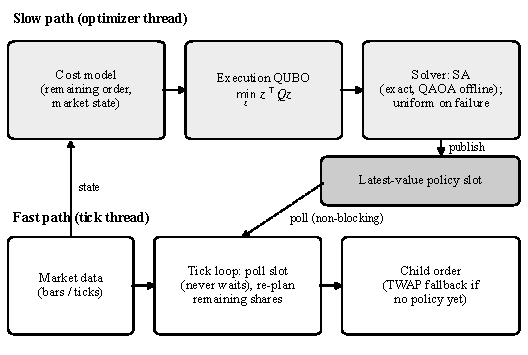
\includegraphics[width=\columnwidth]{fig_paper_architecture.pdf}
\caption{Latency-decoupled hybrid runtime. The slow path rebuilds and solves the execution
QUBO in a background thread and publishes each schedule to a single-slot, lock-protected
mailbox. The fast path polls the slot without waiting, rescales the new schedule's tail to
the shares still unexecuted, and otherwise keeps its current plan (a uniform plan before the
first policy arrives). Solver failures or invalid schedules fall back to a uniform schedule.}
\label{fig:arch}
\end{figure}

Fig.~\ref{fig:arch} shows the runtime and Algorithm~\ref{alg:runtime} its two loops. Its design goal is that the component that submits
child orders never depends on the latency, or the availability, of the optimizer. This is
the property that would make a remote or queue-based quantum solver usable at all in an
execution system.

\emph{Fast path.} A tick thread wakes on a fixed schedule, polls the policy slot, and
submits the child order for the current tick. If a new policy has been published, the fast
path replaces its plan from the current tick onward with the policy's schedule tail,
rescaled and rounded (largest remainder) to the shares not yet executed, so the order
completes exactly after any number of policy switches and never overfills.

\emph{Slow path.} An optimizer thread periodically reads the order state, builds the
execution QUBO, solves it (SA in the runtime; exhaustive search and QAOA are available
offline), validates the schedule and publishes it. Exceptions and invalid schedules trigger a
uniform fallback; the thread never terminates on a solver error.

\begin{algorithm}[t]
\caption{Fast path (one tick) and slow path (one cycle)}
\label{alg:runtime}
\small
\begin{algorithmic}[1]
\Statex \textbf{Fast path}, tick $t$; plan $x$, executed shares $e$, order size $N$
\State $\pi \gets \textsc{PollSlot}()$ \Comment{returns immediately}
\If{$\pi$ is new}
  \State $x_{t:} \gets \textsc{Repair}(\pi_{t:},\ N-e)$ \Comment{rescale, round to sum}
\EndIf
\State submit $\min(x_t,\ N-e)$; update $e$ with the fill
\Statex \textbf{Slow path}, every $\Delta$ seconds
\State read order state; build $Q$ \Comment{no lock held while solving}
\State $z \gets \textsc{Solve}(Q)$; $\pi \gets \textsc{Decode}(z)$
\If{solver failed or $\pi$ invalid} \State $\pi \gets$ uniform schedule \EndIf
\State \textsc{Publish}$(\pi)$ \Comment{overwrite the single slot}
\end{algorithmic}
\end{algorithm}

\emph{Policy slot.} The slot holds only the newest policy and is protected by a lock held for
a few assignments; the consumer never waits for the producer to finish a solve. It is not
lock-free, and the implementation is pure Python (CPython threads), not a kernel-bypass
system. Section~\ref{sec:latency} shows what this costs.

In the real-data evaluation (Section~\ref{sec:results}) the hybrid strategy is simulated
offline: at its re-planning checkpoint it re-solves the remaining units over the remaining
minutes with the same QUBO and SA, after rescaling $\bar V$, $\bar h$ and $\sigma$ by the
ratios observed so far in the same order (bars strictly before the checkpoint), clipped to
$[\HybridClipLow,\HybridClipHigh]$. The frozen setting uses \TuneCheckpoints{} checkpoint. The runtime latency
measurements use the same threads and policy slot with synthetic workloads.

% ======================================================================================
\section{Experimental Protocol}
\label{sec:protocol}

\subsection{Pre-registration and data}

The real-data protocol was written and committed before any market data were downloaded. It
fixes the data, the split, the orders, the strategies, the primary metric, the primary
comparisons, the statistics, the decision rule and the sensitivity analysis; later changes
are listed as deviations in the protocol document, with reasons, and none altered the
primary analysis.

\emph{Data.} Public Binance spot aggregated trades, each daily file verified against its
published SHA-256 checksum, aggregated into one-minute bars (volume, bar VWAP, signed volume
from the taker side, and a trade-sign half-spread estimate). Two symbols were chosen in the
protocol: BTCUSDT, the most liquid USDT pair, and LINKUSDT, chosen before any evaluation as
a pair whose quote volume was in a pre-specified 1--3\% band of BTCUSDT's.

\emph{Split.} \NumDevDays{} development days (\DevFirstDay{} to \DevLastDay) were used for
every estimate and every tuning decision; \NumTestDays{} held-out days (\TestFirstDay{} to
\TestLastDay) were evaluated exactly once, from the clean frozen commit \texttt{\TestCommit}
recorded in the result manifest.

\begin{table}[t]
\caption{Cost-model calibration on development days (OLS impact slope with a day-block
bootstrap standard error; half spread and volatility are means of the intraday profiles).}
\label{tab:calibration}
\centering
\footnotesize
\setlength{\tabcolsep}{3pt}
\begin{tabular}{lrrrrrr}
\toprule
Symbol & ADV & Lot & $\beta$ [SE] & $R^2$ & $\bar h$ (bps) & $\sigma$ (bps)\\
\midrule
BTCUSDT & \BtcAdv{} & \BtcLot & \BtcBeta{} [\BtcBetaSe] & \BtcBetaRsq & \BtcHalfSpread & \BtcSigma\\
LINKUSDT & \LinkAdv{} & \LinkLot & \LinkBeta{} [\LinkBetaSe] & \LinkBetaRsq & \LinkHalfSpread & \LinkSigma\\
\bottomrule
\end{tabular}
\end{table}

\emph{Calibration.} Table~\ref{tab:calibration} summarizes the development-day cost model.
The impact slope comes from a Kyle-style regression, through the origin, of one-minute
returns on signed volume divided by expected volume, over \BtcImpactBars{} bars per symbol.
Its fit is weak ($R^2=\BtcBetaRsq$ and \LinkBetaRsq), which is why the protocol includes an
impact sensitivity analysis. BTCUSDT's half spread is essentially one price tick.

\subsection{Orders, strategies and evaluator}
\label{sec:evaluator}

For each symbol, day and each of \NumStartTimes{} start times four hours apart (from 00:00
UTC; a \emph{window}) we
execute one order in each of \NumCells{} cells: size \EvalSizes{} of development ADV, horizon
\EvalHorizons{} minutes. Sides alternate by start time so that drift does not favour front- or
back-loading. This gives \NumTestWindows{} held-out windows and \NumTestOrders{} orders per
symbol.

Five strategies are compared: TWAP (uniform), VWAP (proportional to the development volume
profile), AC (Section~\ref{sec:ac}), QUBO (Section~\ref{sec:qubo}, solved by SA with
\TuneSweeps{} sweeps and \TuneRestarts{} restarts) and Hybrid (Section~\ref{sec:arch}). No
strategy sees future bars.

Every strategy is executed by the same evaluator. There is no order book for these data, so
the fill model is bar based: a child order for $q$ lots in bar $k$ fills
$\min(q,\lfloor \rho V_k\rfloor)$ lots (a participation cap $\rho=\ParticipationCapPct\%$ of
realized volume $V_k$),
at the bar VWAP moved against the trader by the realized half spread plus
$\beta\,q^{\mathrm{fill}}/V_k$ (linear temporary impact). Unfilled lots carry forward; any
remainder after the last bar is completed by a clean-up order at the same formula without the
cap and charged as opportunity cost, so a strategy cannot look cheaper by not trading. There
is no permanent impact, and fees are omitted because they are the same per unit for every
strategy. Implementation shortfall is measured in bps of arrival notional, positive meaning
cost, and decomposes exactly into spread, impact, timing (price moves before each fill) and
opportunity (clean-up) components.

\subsection{Statistics and decision rule}

The unit of analysis is the window: for each window we average the shortfall difference
\emph{strategy minus baseline} over its \NumCells{} cells. For each of the \NumPrimaryComparisons{} primary comparisons
(QUBO and Hybrid versus TWAP, VWAP and AC, per symbol; $\lambda=0$, impact at 1$\times$) we
report the mean paired difference, a 95\% percentile-bootstrap confidence interval (CI) over
windows (10{,}000 seeded resamples), a day-clustered bootstrap CI, and the two-sided
Wilcoxon signed-rank $p$-value, Holm-adjusted over the \NumPrimaryComparisons{} comparisons. A strategy
\emph{beats} a baseline if the adjusted $p<0.05$ and the mean difference is negative; if the
difference is not significant and its CI lies within $\pm 0.5$~bps we call the two
\emph{practically equivalent}. The sensitivity analysis repeats the evaluation with the
evaluator's impact coefficient at 0.5$\times$ and 2$\times$, with the optimizers either
misspecified (still at 1$\times$) or correctly specified, and is Holm-adjusted jointly over
its \SensNumComparisons{} comparisons. Everything else is exploratory and reported without
adjustment.

\subsection{Synthetic experiments and solver benchmarks}

Before the real-data study, the same strategies were compared on a synthetic market (minute
geometric Brownian motion with an intraday volatility and volume profile, and a synthetic
ten-level book per bar), with \SynSeeds{} seeds per experiment and common random numbers so
that every strategy faces the same book in every minute. These experiments used an earlier
level-encoded QUBO and are reported as a secondary result. Solver benchmarks use the toy
QUBO that was also submitted to IBM hardware, random Gaussian QUBOs, and the binary execution
encoding of Section~\ref{sec:qubo}, with exact bounds by enumeration up to
$n=\SolverMaxN$. QAOA runs on the Qiskit Aer simulator, ideal and with a generic depolarizing
and readout noise model (error rate \QaoaNoise, $n\le\QaoaNoisyMaxN$; not a device
calibration), for depths $p\in\{\QaoaDepths\}$ and \QaoaSeeds{} seeds, optimizing angles with
COBYLA (at most \QaoaMaxIter{} evaluations of \QaoaShots{} shots) and sampling
\QaoaFinalShots{} final shots. The uniform baseline receives the same total budget
(\QaoaShotBudgetMin--\QaoaShotBudgetMax{} shots per run).

% ======================================================================================
\section{Results}
\label{sec:results}

\subsection{Held-out real data}
\label{sec:realdata}

\begin{figure}[t]
\centering
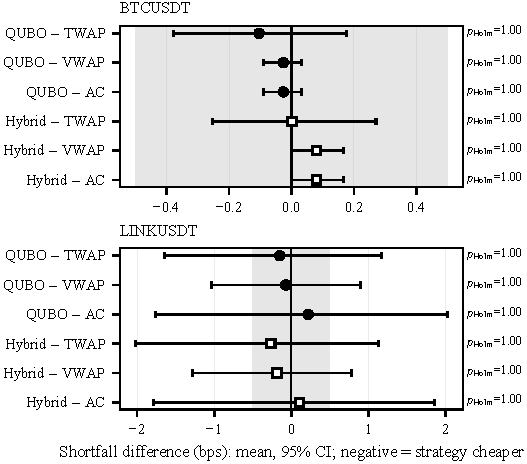
\includegraphics[width=\columnwidth]{fig_paper_primary.pdf}
\caption{The \NumPrimaryComparisons{} pre-registered primary comparisons on \NumTestDays{}
held-out days (\NumTestWindows{} windows per symbol): mean paired shortfall difference with
95\% bootstrap CI and Holm-adjusted $p$. The shaded band is the $\pm 0.5$~bps practical
equivalence margin. Note the different horizontal scales.}
\label{fig:primary}
\end{figure}

\begin{table*}[t]
\caption{Held-out primary comparisons (bps; negative: strategy cheaper). CI: 95\% bootstrap
over windows; day-cluster CI resamples whole days; $p$: two-sided Wilcoxon signed rank;
$p_{\mathrm{Holm}}$: adjusted over the \NumPrimaryComparisons{} comparisons.}
\label{tab:primary}
\centering
\footnotesize
\begin{tabular}{llrrrrr}
\toprule
Symbol & Comparison & Mean & 95\% CI & Day-cluster CI & $p$ & $p_{\mathrm{Holm}}$\\
\midrule
\PrimaryTableRows
\bottomrule
\end{tabular}
\end{table*}

Fig.~\ref{fig:primary} and Table~\ref{tab:primary} give the primary result. None of the
\NumPrimaryComparisons{} comparisons is significant: the smallest Holm-adjusted $p$-value is
\PrimaryMinHolm{} (smallest unadjusted $p$: \PrimaryMinRawP) and the mean differences range
from \PrimaryMinMean{} to \PrimaryMaxMean{}~bps. On BTCUSDT all \BtcNumEquivalent{} CIs lie
within $\pm$\BtcMaxAbsCi{}~bps, so QUBO and Hybrid are practically equivalent to all three
baselines. On LINKUSDT the CIs have a mean half-width of \LinkMeanCiHalfWidth{}~bps and the
result is \emph{no detectable difference}, not equivalence. The in-sample evaluation on the
\NumDevWindows{} development windows per symbol gives the same picture (smallest Holm $p$
\DevMinHolm{}, means \DevMinMean{} to \DevMaxMean{}~bps); on development days every hybrid
variant considered in tuning was \TuneHybridMinusTwapMin--\TuneHybridMinusTwapMax{}~bps
\emph{worse} than TWAP, and the least-bad variant was carried forward as pre-registered.

\emph{Sensitivity.} With the evaluator's impact at 0.5$\times$ or 2$\times$ the calibrated
value, and the optimizers misspecified or correctly specified, no comparison is significant
(smallest jointly adjusted $p$ \SensMinJointHolm; mean differences \SensMinMean{} to
\SensMaxMean~bps). Unadjusted, \SensNumCiExcludeZero{} of the \SensNumComparisons{} CIs
exclude zero, the largest being \SensExclMean{}~bps \SensExclCi, against the hybrid. On
BTCUSDT the 0.5$\times$ and 2$\times$ optimizers produce the same schedules as 1$\times$,
as \eqref{eq:waterfill} predicts for a constant one-tick spread. SA with \RobustnessSeeds{} further seeds
gives identical schedules (spread of the mean differences \RobustnessSpread~bps). In the
exploratory risk-averse variant ($\lambda$ chosen so that $\lambda\Var=\E$ for TWAP), the
front-loaded LINKUSDT schedules differ from TWAP by \RiskLinkQuboTwapMean{}~bps
\RiskLinkQuboTwapCi{} but from the correspondingly risk-averse AC by \RiskLinkQuboAcMean{}~bps
\RiskLinkQuboAcCi; the smallest Holm-adjusted $p$ in that family is \RiskMinHolm.

\begin{table}[t]
\caption{Held-out mean shortfall and components (bps; \NumTestOrders{} orders per symbol).
S+I: spread plus impact; Opp.: clean-up (opportunity) cost; Fill: \% filled before
clean-up; SD: per-order standard deviation of shortfall.}
\label{tab:costs}
\centering
\scriptsize
\setlength{\tabcolsep}{3pt}
\begin{tabular}{llrrrrrr}
\toprule
 & Strategy & IS & S+I & Timing & Opp. & Fill & SD\\
\midrule
\CostTableRows
\bottomrule
\end{tabular}
\end{table}

\begin{figure}[t]
\centering
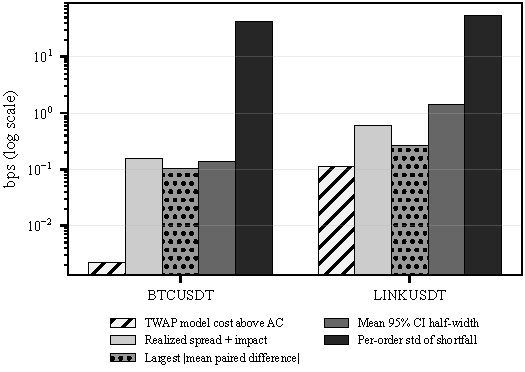
\includegraphics[width=\columnwidth]{fig_paper_signal_vs_noise.pdf}
\caption{Scales on held-out data (log axis). What the choice of schedule can change---the
model-cost advantage of AC over TWAP and the realized spread plus impact---is small compared
with the observed paired differences, their CIs, and above all the per-order standard
deviation of shortfall.}
\label{fig:scales}
\end{figure}

\emph{Why there is no difference.} Table~\ref{tab:costs} and Fig.~\ref{fig:scales} show the
scales involved. Spread plus impact, the part of the cost that a schedule controls, is
\BtcSpreadImpact{}~bps on BTCUSDT and \LinkSpreadImpact{}~bps on LINKUSDT on average, nearly
the same for every strategy. Mean shortfall is \BtcMeanShortfallMin--\BtcMeanShortfallMax{}~bps
on BTCUSDT and \LinkMeanShortfallMin--\LinkMeanShortfallMax{}~bps on LINKUSDT, dominated by
components a schedule barely changes: on BTCUSDT the participation cap binds in thin
minutes (\BtcFillMin--\BtcFillMax\% filled before clean-up), and the clean-up of the
remainder costs \BtcOppMin--\BtcOppMax~bps; on LINKUSDT, timing (price moves during
execution) contributes \LinkTimingMin--\LinkTimingMax~bps. The per-order standard deviation
of shortfall is \BtcStdMin{}~bps on BTCUSDT and \LinkStdMin--\LinkStdMax{}~bps on LINKUSDT.
Even a perfect optimizer of \eqref{eq:objective} could gain little: under the model, the
AC schedule's cost is below TWAP's by only \BtcTwapAcGapMean{}~bps (BTCUSDT) and
\LinkTwapAcGapMean{}~bps (LINKUSDT) on average, about the size of the smallest differences
the design can resolve on BTCUSDT and an order of magnitude below the CI width on LINKUSDT.
Exploratory AC-minus-TWAP differences confirm this: \BtcAcTwapMean{}~bps \BtcAcTwapCi{}
(BTCUSDT) and \LinkAcTwapMean{}~bps \LinkAcTwapCi{} (LINKUSDT).

\begin{figure}[t]
\centering
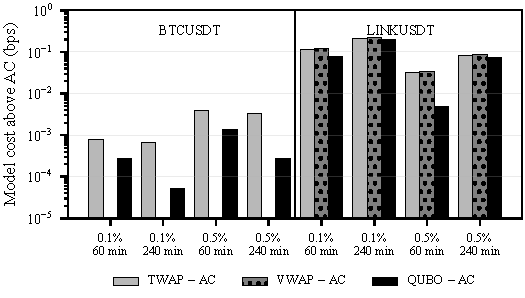
\includegraphics[width=\columnwidth]{fig_paper_qubo_ac_gap.pdf}
\caption{Model cost above discretized AC per order cell (held-out days, mean over windows,
log axis) for TWAP, VWAP and the QUBO schedule found by SA. On BTCUSDT VWAP coincides with AC
(the bar is at the plotting floor). SA reached the exact integer optimum (DP) in every cell,
so the QUBO bars are the cost of the coarse encoding, not solver error.}
\label{fig:gap}
\end{figure}

\emph{QUBO--AC gap.} Fig.~\ref{fig:gap} shows the gap of Section~\ref{sec:qubo} on
held-out cells. SA reached the DP optimum in \QuboAtDpShare\% of cells, with a median solve
time of \QuboSolveTimeMedian~s. The mean gap is \BtcQuboAcGapMean{}~bps on BTCUSDT and
\LinkQuboAcGapMean{}~bps on LINKUSDT (maximum \LinkQuboAcGapMax), smaller than TWAP's excess
in every cell: the QUBO schedule is a slightly worse approximation of AC, as it must be, and
the realized QUBO-minus-AC differences (\BtcQuboAcMean{} and \LinkQuboAcMean{}~bps) are
consistent with that and with zero.

\subsection{Synthetic market}
\label{sec:synthetic}

\begin{figure}[t]
\centering
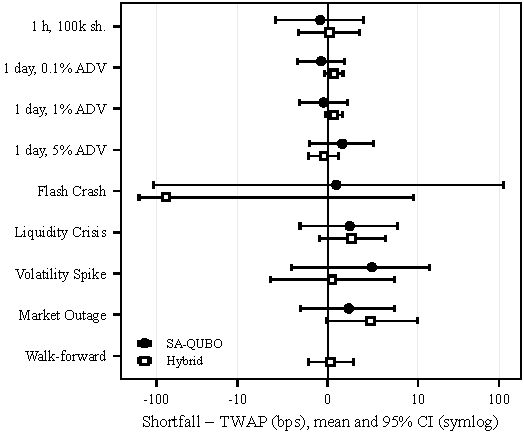
\includegraphics[width=\columnwidth]{fig_paper_synthetic.pdf}
\caption{Synthetic market, \SynSeeds{} seeds per setting: shortfall difference against TWAP
(mean and 95\% bootstrap CI, symmetric-log axis) of the SA-QUBO and hybrid schedules in every
strategy experiment. The walk-forward experiment has no static QUBO arm.}
\label{fig:synthetic}
\end{figure}

Fig.~\ref{fig:synthetic} summarizes the synthetic experiments. In no setting does a CI
exclude zero in favour of SA-QUBO or the hybrid against TWAP. For one simulated hour
(\SynHourShares{} shares) the hybrid differs from TWAP by \SynHourHybridTwapMean{}~bps
\SynHourHybridTwapCi{} ($p=\SynHourHybridTwapP$) and SA-QUBO by \SynHourQuboTwapMean{}~bps
\SynHourQuboTwapCi; in the walk-forward backtest the hybrid differs by
\SynWfHybridTwapMean{}~bps \SynWfHybridTwapCi. At 1\% of daily volume the QUBO schedules pay
slightly \emph{more} impact than TWAP (hybrid \SynDayImpactHybridTwapMean{}~bps
\SynDayImpactHybridTwapCi; SA-QUBO \SynDayImpactQuboTwapMean{}~bps
\SynDayImpactQuboTwapCi) because the discrete quantity levels of the earlier encoding make
the schedule lumpier. The only significant difference in the stress scenarios is against the
hybrid: in a simulated market outage it is \SynOutageHybridVwapMean{}~bps
\SynOutageHybridVwapCi{} worse than VWAP ($p=\SynOutageHybridVwapP$, unadjusted). The large
flash-crash effects are price-path luck (any schedule that trades later pays less), not an
optimizer property.

\subsection{Solvers and QAOA}
\label{sec:solvers}

\begin{figure}[t]
\centering
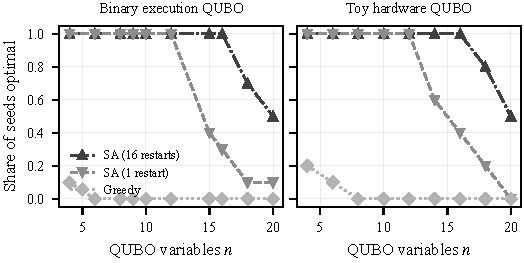
\includegraphics[width=\columnwidth]{fig_paper_solver_success.pdf}
\caption{Share of \SolverSeeds{} seeds in which each classical heuristic returns the exact
optimum (by enumeration), on the binary execution encoding and on the toy QUBO submitted to
hardware. SA: \TuneSweeps{} sweeps, geometric schedule; \TuneRestarts{} restarts or one.}
\label{fig:sa}
\end{figure}

\emph{Classical solvers.} An earlier version of our SA ignored its sweep budget and stopped
early; with that defect it found the optimum of the toy QUBO in only a small
minority of seeds, which made quantum solvers look competitive. After the fix (exactly
\TuneSweeps{} sweeps at geometrically spaced temperatures with bounds set from the QUBO's
coefficients, and vectorized restarts), SA with \TuneRestarts{} restarts finds the exact optimum in every
seed up to $n=\SaSliceAllOptimalUpTo$ on the binary execution encoding and up to
$n=\SaToyAllOptimalUpTo$ on the toy QUBO, and in \SaSliceAboveMin--\SaSliceAboveMax\% and
\SaToyAboveMin--\SaToyAboveMax\% of seeds at $n={}$\SaSliceAboveSizes{} (Fig.~\ref{fig:sa}); a greedy
descent is optimal in at most \GreedyToyMax\% of seeds. SA takes \SaTimeMin--\SaTimeMax~s per
solve, and exhaustive search \BruteForceTimeMaxN~s at $n=\SolverMaxN$. On the real-data
instances the question does not arise: $n=\TuneVariables$ is solved exactly by DP.

\begin{figure*}[t]
\centering
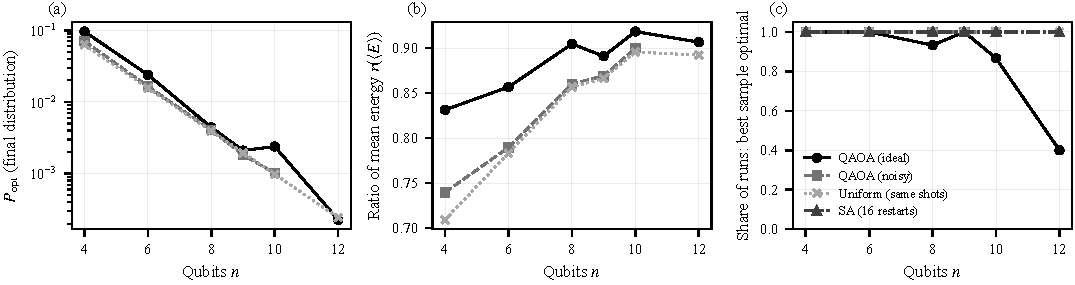
\includegraphics[width=\textwidth]{fig_paper_qaoa.pdf}
\caption{QAOA on the binary execution encoding (ideal and noisy Aer simulators; mean over
depths $p\in\{\QaoaDepths\}$ and seeds) against a uniform random sampler with the same total shot budget.
(a)~Success probability of the final distribution (log axis). (b)~Approximation ratio of the
mean energy. (c)~Share of runs in which the best sample is optimal; uniform sampling and SA
are optimal in every run, so this metric cannot distinguish the solvers at these sizes.}
\label{fig:qaoa}
\end{figure*}

\begin{table}[t]
\caption{QAOA minus same-budget uniform sampling. $\Delta\Popt$: success-probability
difference with 95\% bootstrap CI; $p$: Wilcoxon, unadjusted; $\Delta r$: difference in
the mean-energy ratio; last column: \% of runs whose best sample is optimal, QAOA / uniform.
Instance: one level-encoded execution QUBO, $n=\InstanceN$.}
\label{tab:qaoa}
\centering
\scriptsize
\setlength{\tabcolsep}{2.5pt}
\begin{tabular}{llrlrrr}
\toprule
Family & Sim. & Runs & $\Delta\Popt$ [95\% CI] & $p$ & $\Delta r$ & Best opt.\\
\midrule
\QaoaTableRows
\bottomrule
\end{tabular}
\end{table}

\emph{QAOA.} Table~\ref{tab:qaoa} and Fig.~\ref{fig:qaoa} compare QAOA with the uniform
baseline. On the toy and random families, ideal QAOA places a small but significant
additional probability on the optimum (\QaoaToyIdealPoptMean{} \QaoaToyIdealPoptCi{} and
\QaoaRandomIdealPoptMean{} \QaoaRandomIdealPoptCi, unadjusted $p=\QaoaToyIdealPoptP$ and
\QaoaRandomIdealPoptP); the largest per-cell value is $\Popt=\QaoaToyBestCellPopt$ at
$n=\QaoaToyBestCellN$, $p=\QaoaToyBestCellP$, against \QaoaToyBestCellUniform{} for uniform
sampling. On the binary execution encoding the advantage is not significant
(\QaoaSliceIdealPoptMean{} \QaoaSliceIdealPoptCi, $p=\QaoaSliceIdealPoptP$; noisy
\QaoaSliceNoisyPoptMean{} \QaoaSliceNoisyPoptCi) and it fades with $n$: at $n=4$ ideal QAOA
reaches \QaoaSliceNFourPopt{} against \QaoaSliceNFourUniform, at $n=12$ \QaoaSliceNOneTwoPopt{}
against \QaoaSliceNOneTwoUniform. The mean energy is consistently better than uniform
($\Delta r$ between \QaoaEnergyMin{} and \QaoaEnergyMax), i.e., QAOA
shifts probability toward low energies without concentrating it on the optimum. The noise
model does not act as a uniform discount: across families, sizes and depths the ratio of
noisy to ideal $\Popt$ ranges from \NoiseRatioMin{} to \NoiseRatioMax.

\emph{Best-of-shots metrics are uninformative here.} The share of runs whose best sample is
optimal is \QaoaSliceIdealBestOpt\% for ideal QAOA on the binary encoding and \QaoaSliceIdealUniformBestOpt\% for uniform
sampling with the same budget. This is arithmetic, not a quantum effect: with
$S\ge\QaoaShotBudgetMin$ shots, uniform sampling misses a unique optimum at $n=\QaoaMaxN$ with
probability $(1-2^{-n})^S$, i.e., \UniformMissProbMaxN. Any QAOA study whose shot budget is comparable to or larger than $2^n$ and that
reports the best sampled bitstring, or an approximation ratio computed from it, therefore
measures the shot budget. On the single level-encoded instance with $n=\InstanceN$, SA found the
optimum in \InstanceSaOptimal{} seeds in \InstanceSaTime~s, while ideal QAOA took
\InstanceQaoaTimeMin--\InstanceQaoaTimeMax~s of simulation. The QUBO-to-Ising mapping itself
is exact: over \IsingSamples{} random QUBOs per size for $n=\IsingMinN$--\IsingMaxN, the
largest relative energy error was \IsingMaxRelError.

\subsection{Latency}
\label{sec:latency}

\begin{figure}[t]
\centering
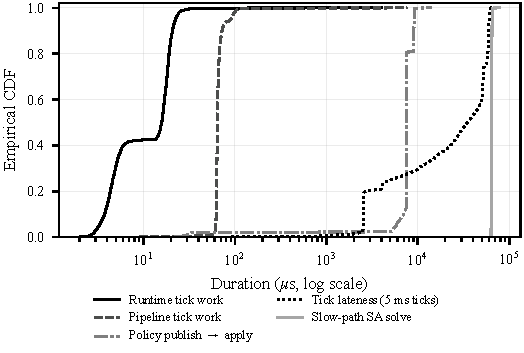
\includegraphics[width=\columnwidth]{fig_paper_latency.pdf}
\caption{Empirical CDFs of runtime durations (\LatencyCpu, CPython \LatencyPython; log axis).
The fast path's own work takes microseconds, but because the pure-Python SA solve holds the
interpreter lock, ticks scheduled every \TickIntervalMs~ms start tens of milliseconds late.}
\label{fig:latency}
\end{figure}

\begin{table}[t]
\caption{Measured runtime latencies (\LatencyCpu, CPython \LatencyPython).}
\label{tab:latency}
\centering
\scriptsize
\setlength{\tabcolsep}{3pt}
\begin{tabular}{p{0.52\columnwidth}rrrl}
\toprule
Component & Samples & Median & p99 & Unit\\
\midrule
\LatencyTableRows
\bottomrule
\end{tabular}
\end{table}

Table~\ref{tab:latency} and Fig.~\ref{fig:latency} report latencies measured with a
monotonic clock. The fast path's own work per tick is small (median \RuntimeTickMedian{} and
p99 \RuntimeTickPtt~$\mu$s in the runtime; \PipelineTickMedian{} and \PipelineTickPtt~$\mu$s
in a pipeline that also updates microstructure estimators), and the fast path never waits
for a solve. It is nevertheless \emph{delayed} by it: with \TickIntervalMs~ms ticks and a
slow path that re-solves every \OptimizerIntervalMs~ms, ticks start a median
\TickLatenessMedian~ms (p99 \TickLatenessPtt~ms) after their scheduled time, because the SA
solve (median \RuntimeSolveMedian~ms for the runtime QUBO) holds CPython's global interpreter
lock. A published policy reaches the fast path after a median \PropagationMedian~ms. Under
load, \LoadOrders{} concurrent orders on \LoadConcurrency{} threads completed in
\LoadWallTime~s, all filled completely, with a median \LoadOverheadMedian~s of overhead over
the tick schedule. The decoupling therefore protects correctness (orders complete, never
overfill, and never wait for a policy) but not timeliness in a single Python process; a
production design would run the optimizer in a separate process or service.

\subsection{IBM quantum hardware}
\label{sec:hardware}

\emph{Data.} QAOA was run on IBM's \texttt{ibm\_fez} processor on \HwDate{} for the toy
QUBO of Section~\ref{sec:solvers}, at $n=\HwMinN$ and $n=\HwMaxN$ only, with \HwRunsPerN{}
runs per size and the configured depth $p=1$ (the depth is not recorded in the job data).
Each run optimized the two angles with COBYLA on \HwLoopShots-shot jobs
(\HwLoopJobsMin--\HwLoopJobsMax{} per run) and ended with one \HwFinalShots-shot job at the
final angles. The records committed with the earlier draft of this work are not usable as
evidence: their count tables are empty and their derived fields are inconsistent with them.
They also listed one run each at $n=6$ and $n=8$; these could not be matched to any job on
the account. We therefore recovered the raw counts of every job on the account from IBM
Quantum: \HwNumRecords{} records for \HwNumUniqueJobs{} jobs, of which \HwNumJobs{}
completed with counts and \HwNumExcluded{} were cancelled while queued. Every energy is
recomputed from the counts with the known QUBO (Qiskit bit order, checked by a test). Loop
and final jobs are told apart by their shot counts, and loop jobs are assigned to runs per
size by creation time: the runs of one size ran one after another, while the two sizes were
interleaved. The \HwNumIncompleteJobs{} loop jobs created after the last final job
(\HwNFourIncomplete{} at $n=4$, \HwNOneZeroIncomplete{} at $n=10$) belong to a fourth run
per size that has no final job; they appear in Fig.~\ref{fig:hwtraj} but not in the
statistics.

\emph{Statistics.} For each final job we report the success probability $\Popt$ with a
Wilson 95\% interval and a one-sided exact binomial test against uniform sampling (the
optimum is unique at both sizes, so $\Popt^{\mathrm{unif}}=2^{-n}$), and the approximation
ratio $r$ of the mean energy minus its exact uniform value, with a shot-level bootstrap 95\%
interval (\HwBootstrap{} multinomial resamples). These intervals describe shot noise within
one job. Runs differ by far more than shot noise (different random starting angles, device
drift), so we report each run and the range over runs rather than pooling them. Three runs
per size is small: even three runs out of three on the same side of uniform sampling give
only $p=\HwSignP$ by a sign test.

\begin{table}[t]
\caption{IBM \texttt{ibm\_fez}, $p=1$ QAOA on the toy QUBO: final jobs of \HwFinalShots{}
shots. $\Popt$ with Wilson 95\% CI; $p_>$: one-sided exact binomial test of
$\Popt>2^{-n}$, unadjusted; $r$: approximation ratio of the mean energy; $\Delta r$: $r$
minus its uniform value, with shot-bootstrap 95\% CI. Rows ``unif.'': exact values for
uniform sampling.}
\label{tab:hw}
\centering
\scriptsize
\setlength{\tabcolsep}{1.7pt}
\begin{tabular}{rllrrl}
\toprule
$n$ & Run & $\Popt$ [95\% CI] & $p_>$ & $r$ & $\Delta r$ [95\% CI]\\
\midrule
\HwTableRows
\bottomrule
\end{tabular}
\end{table}

\begin{figure}[t]
\centering
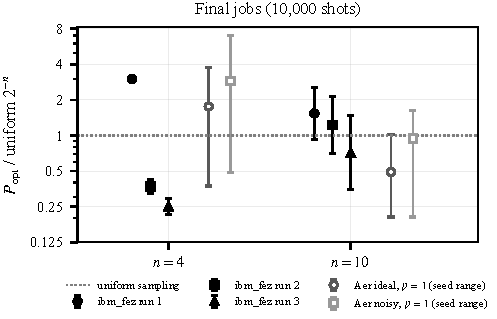
\includegraphics[width=\columnwidth]{fig_hw_ibm_success_prob.pdf}\\[2pt]
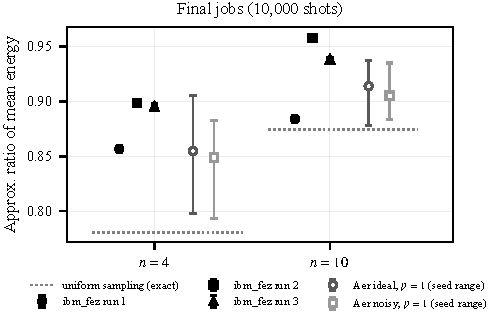
\includegraphics[width=\columnwidth]{fig_hw_ibm_approx_ratio.pdf}
\caption{Final \texttt{ibm\_fez} jobs, one marker per run, next to the Aer $p=1$ results on
the same QUBO (mean and range over \HwNFourIdealSeeds{} seeds). Top: $\Popt$ relative to
uniform sampling (log axis; Wilson 95\% CIs). Bottom: approximation ratio of the mean energy
(bootstrap CIs are smaller than the markers); dotted: exact uniform value.}
\label{fig:hw}
\end{figure}

\begin{figure}[t]
\centering
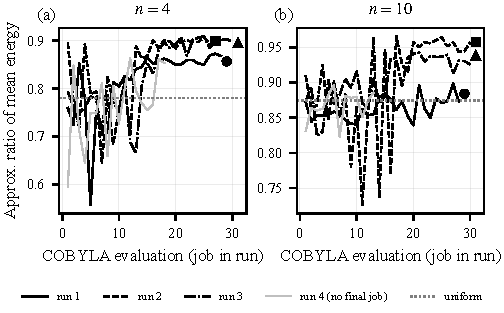
\includegraphics[width=\columnwidth]{fig_hw_ibm_trajectory.pdf}
\caption{COBYLA on \texttt{ibm\_fez}: approximation ratio of the mean energy of each
\HwLoopShots-shot loop job by position in its run; the final job of each run is the marker at
the end. Gray: the fourth run of each size, which has no final job.}
\label{fig:hwtraj}
\end{figure}

\emph{Mean energy.} Every final job has a lower mean energy than uniform sampling, with
bootstrap intervals that exclude zero (Table~\ref{tab:hw}): $\Delta r$ is
\HwNFourAdvMin--\HwNFourAdvMax{} at $n=4$ and \HwNOneZeroAdvMin--\HwNOneZeroAdvMax{} at
$n=10$ (all three runs above uniform at both sizes). The ratios,
\HwNFourRatioMin--\HwNFourRatioMax{} and \HwNOneZeroRatioMin--\HwNOneZeroRatioMax, are
comparable to those of the Aer simulators at $p=1$ (means \HwNFourIdealRatio{} and
\HwNOneZeroIdealRatio{} ideal, \HwNFourNoisyRatio{} and \HwNOneZeroNoisyRatio{} noisy;
Fig.~\ref{fig:hw}). The simulator runs used fewer shots per evaluation
(Section~\ref{sec:protocol}), so this comparison says that the device did not prevent
COBYLA from finding useful angles, not that it matches an ideal device. The optimization
itself worked on hardware: in every complete run, the mean ratio of the last five loop jobs
(\HwNFourLastFiveMin--\HwNFourLastFiveMax{} at $n=4$,
\HwNOneZeroLastFiveMin--\HwNOneZeroLastFiveMax{} at $n=10$) exceeds that of the first five
(\HwNFourFirstFiveMin--\HwNFourFirstFiveMax{} and
\HwNOneZeroFirstFiveMin--\HwNOneZeroFirstFiveMax; Fig.~\ref{fig:hwtraj}), although one
$n=10$ run stayed close to the uniform value throughout.

\emph{Probability of the optimum.} Here the evidence for any advantage is weak. At $n=4$,
one run placed $\Popt=\HwNFourPoptMax$ on the optimum, \HwNFourPoptMaxRatio{} times the
uniform \HwNFourUniform{} ($p_>$\,\HwNFourPMin), but the other two placed \HwNFourPoptMid{} and
\HwNFourPoptMin, significantly \emph{below} the uniform value (one-sided exact test,
$p$\,\HwNFourPLessMax); the run with the highest
$\Popt$ has the lowest mean-energy ratio, so the angles found trade concentration on the
optimum against low energy overall. At $n=10$, \HwNOneZeroRunsAbove{} of three runs are
above $2^{-10}$ but none significantly ($p_>=\HwNOneZeroPMin$ to \HwNOneZeroPMax), with
$\Popt$ between \HwNOneZeroPoptMin{} and \HwNOneZeroPoptMax{} against \HwNOneZeroUniform. The
spread between runs is of the same order as the spread between simulator seeds (ideal Aer
at $n=4$: \HwNFourIdealPoptMin--\HwNFourIdealPoptMax), so it need not come from the
device: different starting angles alone produce a spread this large in simulation. The optimum was sampled in every final job, but,
as in Section~\ref{sec:solvers}, this carries no information: uniform sampling with
\HwFinalShots{} shots misses it with probability \HwNOneZeroUniformMiss{} at $n=10$.

\emph{No advantage over classical solvers.} Both sizes are solved exactly by enumeration and
by SA in every seed (Section~\ref{sec:solvers}; \SaTimeMin--\SaTimeMax~s per SA solve). The
hardware returned a distribution with better-than-random mean energy, not a better solution.
A complete run spanned \HwRunSpanMin--\HwRunSpanMax~s from its first to its last job
creation, with a median of \HwJobIntervalMedian~s between consecutive jobs of a run; these
are wall-clock intervals that include queueing and the classical loop, not QPU time. Neither
the QPU time nor the cost of the runs is recorded in the recovered data, so we report
neither.

\emph{Data.} The raw counts are in \url{results/ibm_fez_recovered.jsonl}; the IDs of all
analysed, final, incomplete-run and excluded jobs are listed in
\url{results/hardware/manifest.json}.

% ======================================================================================
\section{Discussion: When Could Quantum Optimization Help?}
\label{sec:discussion}

The negative result has a simple structure. The execution problem studied here is a small,
convex-in-the-relaxation program with a chain structure: discretized AC solves the continuous
version exactly, DP solves the integer version exactly, and a correctly
implemented SA finds the QUBO optimum reliably. A quantum solver cannot improve on an exact
solution, and on liquid markets even the exact solution is worth a fraction of a basis point
relative to TWAP. The following are \emph{hypotheses}, not findings, about where these
conditions fail; each would need its own pre-registered test.

\begin{enumerate}
\item \emph{Costs large relative to noise.} The controllable cost scales with the order's
  participation rate and with how uneven the liquidity profile is. Illiquid assets and
  orders that are large relative to average daily volume would raise the stakes of
  scheduling; whether that makes differences detectable depends on how the price noise
  scales with the horizon.
\item \emph{Genuinely combinatorial structure.} Multi-venue lot allocation, minimum-fill and
  odd-lot rules, fee tiers, and portfolio transitions with cardinality or round-lot
  constraints break the chain structure that makes our program easy. Only in such instances,
  and only when exact methods (mixed-integer programming, DP) and well-tuned SA stop
  scaling, is there room for any heuristic, quantum or classical, to add value.
\item \emph{Sizes beyond enumeration, with fair baselines.} At $n\le\QaoaMaxN$ any sampler
  with thousands of shots finds the optimum by chance. Evidence of a quantum contribution
  requires sizes where uniform sampling and exhaustive search fail, a comparison at equal
  wall-clock and shot budgets, and the success probability or the mean energy rather than
  the best sample.
\item \emph{Latency compatibility.} The decoupled architecture tolerates slow solves, but a
  schedule is only useful if it arrives within the re-planning interval. Remote quantum
  execution adds queueing, transpilation and communication delays: on \texttt{ibm\_fez}, a
  median of \HwJobIntervalMedian~s passed between consecutive jobs of a QAOA run, and a
  complete run took \HwRunSpanMin--\HwRunSpanMax~s (Section~\ref{sec:hardware}), against
  the \OptimizerIntervalMs~ms re-solve interval of our runtime.
\end{enumerate}

\subsection*{Lessons from auditing the earlier draft}

Four problems in the earlier version of this work are common enough to be worth stating as
lessons, because each one made the quantum approach look better than it is.
\begin{enumerate}
\item \emph{Unequal execution models.} Strategies were executed by different fill models,
  so part of the reported advantage came from the simulator rather than the schedule. Every
  comparison now uses one evaluator, common random numbers and an opportunity cost for
  unfilled shares.
\item \emph{A weakened classical baseline.} The annealer silently ignored its sweep budget.
  Benchmarks of quantum heuristics should verify that the classical baseline receives the
  budget it is said to receive, and should compare against an exact solution where one is
  available.
\item \emph{Saturating metrics.} Best-of-shots approximation ratios were reported as solution
  quality; at small $n$ they measure the shot budget (Section~\ref{sec:solvers}).
\item \emph{Numbers without provenance.} Some figures were drawn from typed-in values, and
  hardware results were kept without raw counts. The repository now forbids both: figures
  read only result files, the paper's numbers are generated, and hardware claims require
  recoverable job identifiers and counts.
\end{enumerate}

% ======================================================================================
\section{Limitations and Threats to Validity}
\label{sec:limitations}

\emph{Market model.} The real-data evaluator is bar based: no limit-order book, no queue
position, no permanent impact, no fees, a linear impact coefficient from a regression with
$R^2=\BtcBetaRsq$ (BTCUSDT) and \LinkBetaRsq{} (LINKUSDT), and a half-spread estimate from
trade signs. No level-2 data were used. The synthetic experiments use an uncalibrated
simulator and a synthetic book, and an earlier level encoding of the QUBO. Different fill
models could change the size of the costs, although the order-of-magnitude gap between
controllable cost and price noise is unlikely to close for these symbols.

\emph{Scope.} Two crypto spot pairs, \NumDevDays{} development and \NumTestDays{} test days,
two order sizes and two horizons. Results for equities, futures or illiquid assets may
differ.

\emph{Construct validity.} Shortfall includes a clean-up charge for lots the participation
cap left unfilled. On BTCUSDT this component dominates the mean, and it is only weakly
affected by the schedule; a different cap would shift levels, not the comparison, because
all strategies face the same cap.

\emph{Problem size and solvers.} The real-data QUBO has \TuneVariables{} variables and is
solved exactly by DP; QAOA was simulated only up to $n=\QaoaMaxN$, with a generic noise
model rather than a device calibration, and run on hardware only at $n=4$ and $n=10$ with
three runs each, at one depth, on one device and one day. The \emph{hybrid} strategy's
re-planning rule was selected on development days although every variant was worse than
TWAP there; a different adaptive rule might behave differently.

\emph{Latency.} All latencies are CPython-thread measurements on one laptop-class machine;
they characterize this implementation, not the architecture's limits.

\emph{Internal validity.} The protocol, the split and the decision rule were fixed in
advance; tuning used development days only; the held-out run was executed once from a clean
commit (\texttt{\TestCommit}). The development-day evaluation was recorded from a working
tree marked \emph{\DevCommitClean} in its manifest (commit \texttt{\DevCommit}); it is
in-sample by design and not part of the confirmatory result. Deviations from the protocol
are listed, with reasons, in the repository.

% ======================================================================================
\section{Reproducibility}
\label{sec:repro}

The code, results and manuscript sources are available at
\url{https://github.com/Quantum-Blade1/Hybrid-Quantum-Classical-Optimal-Execution-Engine-for-Low-Latency-Trading}
under the Apache~2.0 license. \texttt{make all} downloads the public Binance files (verified
against their published checksums), runs every experiment, draws every figure and writes the
number macros used in this paper; \texttt{make quick} runs everything at tiny sizes, as the
continuous-integration job does. Each experiment writes a
\texttt{manifest.json} with its configuration, seeds, commit hash and dirty flag, package
versions, platform, wall time and the SHA-256 of every output file. A figure registry maps
each figure to the function that draws it and the result files it reads, and a test enforces
that figure code reads results only. The file \texttt{numbers.tex} is generated from the
committed results, and \texttt{make check-paper} fails if it is stale. The pre-registered
protocol, a ledger of every claim of the earlier draft and its fate, and a summary of all
results are in \texttt{docs/}.

% ======================================================================================
\section{Conclusion}
\label{sec:conclusion}

We built a hybrid quantum--classical execution system with a fast path that never waits for
the optimizer and an exact binary QUBO encoding of the discretized execution problem, and
evaluated it under a pre-registered protocol on held-out Binance data. The QUBO and hybrid
schedules are not distinguishable from TWAP, VWAP or discretized Almgren--Chriss, on BTCUSDT
within half a basis point, and the reason is that the costs a schedule controls are small
compared with the price noise it does not. On the solver side, a correct classical annealer
solves every real-data instance and every benchmark instance up to
$n=\SaSliceAllOptimalUpTo$, and QAOA on simulators does not beat uniform sampling at
finding the optimum of the binary execution encoding. On IBM hardware, $p=1$ QAOA at $n=4$
and $n=10$ lowered the mean energy below that of uniform sampling in every run but did not
reliably raise the probability of the optimum. The contribution is therefore a
reproducible system, an evaluation method, and a clear statement of what a quantum optimizer
would have to demonstrate, on which problems, to matter for trade execution.

\section*{Acknowledgment}
The authors thank IBM Quantum for access to the \texttt{ibm\_fez} system through its open
plan. % TODO(author): confirm funding and acknowledgment text before submission.

% ======================================================================================
\begin{thebibliography}{99}

\bibitem{perold1988}
A.~F. Perold, ``The implementation shortfall: Paper versus reality,'' \emph{J. Portfolio
Manage.}, vol.~14, no.~3, pp.~4--9, 1988.

\bibitem{bertsimas1998}
D.~Bertsimas and A.~W. Lo, ``Optimal control of execution costs,'' \emph{J. Financial
Markets}, vol.~1, no.~1, pp.~1--50, 1998.

\bibitem{almgren2001}
R.~Almgren and N.~Chriss, ``Optimal execution of portfolio transactions,'' \emph{J. Risk},
vol.~3, no.~2, pp.~5--39, 2001.

\bibitem{lucas2014}
A.~Lucas, ``Ising formulations of many NP problems,'' \emph{Front. Phys.}, vol.~2, p.~5,
2014.

\bibitem{kadowaki1998}
T.~Kadowaki and H.~Nishimori, ``Quantum annealing in the transverse Ising model,''
\emph{Phys. Rev. E}, vol.~58, no.~5, p.~5355, 1998.

\bibitem{farhi2014}
E.~Farhi, J.~Goldstone, and S.~Gutmann, ``A quantum approximate optimization algorithm,''
arXiv:1411.4028, 2014.

\bibitem{rosenberg2016}
G.~Rosenberg, P.~Haghnegahdar, P.~Goddard, P.~Carr, K.~Wu, and M.~L{\'o}pez de Prado,
``Solving the optimal trading trajectory problem using a quantum annealer,'' \emph{IEEE J.
Sel. Topics Signal Process.}, vol.~10, no.~6, pp.~1053--1060, 2016.

\bibitem{orus2019}
R.~Or{\'u}s, S.~Mugel, and E.~Lizaso, ``Quantum computing for finance: Overview and
prospects,'' \emph{Rev. Phys.}, vol.~4, p.~100028, 2019.

\bibitem{egger2020}
D.~J. Egger, C.~Gambella, J.~Marecek, S.~McFaddin, M.~Mevissen, R.~Raymond, A.~Simonetto,
S.~Woerner, and E.~Yndurain, ``Quantum computing for finance: State-of-the-art and future
prospects,'' \emph{IEEE Trans. Quantum Eng.}, vol.~1, pp.~1--24, 2020.

\bibitem{almgren2005}
R.~Almgren, C.~Thum, E.~Hauptmann, and H.~Li, ``Direct estimation of equity market impact,''
\emph{Risk}, vol.~18, no.~7, pp.~58--62, 2005.

\bibitem{gueant2012}
O.~Gu{\'e}ant, C.-A. Lehalle, and J.~Fernandez-Tapia, ``Optimal portfolio liquidation with
limit orders,'' \emph{SIAM J. Financial Math.}, vol.~3, no.~1, pp.~740--764, 2012.

\bibitem{forsyth2012}
P.~A. Forsyth, J.~S. Kennedy, S.~T. Tse, and H.~Windcliff, ``Optimal trade execution: A mean
quadratic variation approach,'' \emph{J. Econ. Dyn. Control}, vol.~36, no.~12,
pp.~1971--1991, 2012.

\bibitem{cont2017}
R.~Cont and A.~Kukanov, ``Optimal order placement in limit order markets,'' \emph{Quant.
Finance}, vol.~17, no.~1, pp.~21--39, 2017.

\bibitem{ning2021}
B.~Ning, F.~H.~T. Lin, and S.~Jaimungal, ``Double deep Q-learning for optimal execution,''
\emph{Appl. Math. Finance}, vol.~28, no.~4, pp.~361--380, 2021.

\bibitem{cartea2015}
{\'A}.~Cartea, S.~Jaimungal, and J.~Penalva, \emph{Algorithmic and High-Frequency
Trading}. Cambridge, U.K.: Cambridge Univ. Press, 2015.

\bibitem{brandhofer2023}
S.~Brandhofer \emph{et al.}, ``Benchmarking the performance of portfolio optimization with
QAOA,'' \emph{Quantum Inf. Process.}, vol.~22, p.~25, 2023.

\bibitem{braine2021}
L.~Braine, D.~J. Egger, J.~Glick, and S.~Woerner, ``Quantum algorithms for mixed binary
optimization applied to transaction settlement,'' \emph{IEEE Trans. Quantum Eng.}, vol.~2,
pp.~1--8, 2021.

\bibitem{stamatopoulos2020}
N.~Stamatopoulos, D.~J. Egger, Y.~Sun, C.~Zoufal, R.~Iten, N.~Shen, and S.~Woerner,
``Option pricing using quantum computers,'' \emph{Quantum}, vol.~4, p.~291, 2020.

\bibitem{woerner2019}
S.~Woerner and D.~J. Egger, ``Quantum risk analysis,'' \emph{npj Quantum Inf.}, vol.~5,
p.~15, 2019.

\bibitem{egger2021credit}
D.~J. Egger, R.~Garc{\'i}a Guti{\'e}rrez, J.~Cahu{\'e} Mestre, and S.~Woerner, ``Credit
risk analysis using quantum computers,'' \emph{IEEE Trans. Comput.}, vol.~70, no.~12,
pp.~2136--2145, 2021.

\bibitem{kyle1985}
A.~S. Kyle, ``Continuous auctions and insider trading,'' \emph{Econometrica}, vol.~53,
no.~6, pp.~1315--1335, 1985.

\bibitem{glosten1985}
L.~R. Glosten and P.~R. Milgrom, ``Bid, ask and transaction prices in a specialist market
with heterogeneously informed traders,'' \emph{J. Financial Econ.}, vol.~14, no.~1,
pp.~71--100, 1985.

\bibitem{ohara1995}
M.~O'Hara, \emph{Market Microstructure Theory}. Cambridge, MA, USA: Blackwell, 1995.

\bibitem{wilcoxon1945}
F.~Wilcoxon, ``Individual comparisons by ranking methods,'' \emph{Biometrics Bull.},
vol.~1, no.~6, pp.~80--83, 1945.

\bibitem{holm1979}
S.~Holm, ``A simple sequentially rejective multiple test procedure,'' \emph{Scand. J.
Statist.}, vol.~6, no.~2, pp.~65--70, 1979.

\bibitem{kirkpatrick1983}
S.~Kirkpatrick, C.~D. Gelatt, and M.~P. Vecchi, ``Optimization by simulated annealing,''
\emph{Science}, vol.~220, no.~4598, pp.~671--680, 1983.

\end{thebibliography}

\end{document}
